\documentclass[a4paper,USenglish,cleveref, autoref,anonymous]{lipics-v2021}

%% final papers: 25 pages

%This is a template for producing LIPIcs articles. 
%See lipics-v2021-authors-guidelines.pdf for further information.
%for A4 paper format use option "a4paper", for US-letter use option "letterpaper"
%for british hyphenation rules use option "UKenglish", for american hyphenation rules use option "USenglish"
%for section-numbered lemmas etc., use "numberwithinsect"
%for enabling cleveref support, use "cleveref"
%for enabling autoref support, use "autoref"
%for anonymousing the authors (e.g. for double-blind review), add "anonymous"
%for enabling thm-restate support, use "thm-restate"
%for enabling a two-column layout for the author/affilation part (only applicable for > 6 authors), use "authorcolumns"
%for producing a PDF according the PDF/A standard, add "pdfa"

\pdfoutput=1 %uncomment to ensure pdflatex processing (mandatatory e.g. to submit to arXiv)
%\hideLIPIcs  %uncomment to remove references to LIPIcs series (logo, DOI, ...), e.g. when preparing a pre-final version to be uploaded to arXiv or another public repository

%\graphicspath{{./graphics/}}%helpful if your graphic files are in another directory
\usepackage{microtype}%if unwanted, comment out or use option "draft"
\pdfoutput=1
\usepackage[utf8]{inputenc}
\usepackage{amsmath}
\usepackage{amssymb}
\usepackage{mathpartir}
\usepackage{hyperref}
\usepackage{listings}
\usepackage{graphicx}
\usepackage{comment}
\usepackage{todonotes}
\newcommand\pt{\todo[author=PT,inline]}
\newcommand\atha{\todo[author={@Ha},inline]}
\lstdefinelanguage{michelson}{
  basicstyle=\fontsize{8}{9.6}\selectfont,
  morekeywords={parameter,storage,or,unit,mutez,pair,bool,address}, sensitive=false,
  morecomment=[l]{\#},
  morecomment=[\STACK]{/*}{*/},
  morestring=[b]",
}
\lstset{
  language=Caml,
  captionpos=b,
  aboveskip=-\smallskipamount,
  belowskip=-\smallskipamount,
  belowcaptionskip=0pt,
  basicstyle=\fontsize{8}{9.6}\selectfont,
  morekeywords={val}
}

%% structure
\newcommand{\Angle}[1]{\langle#1\rangle}

%% values
\newcommand{\NEG}{\neg}
\newcommand{\CNF}{\wedge}
\newcommand{\DNF}{\vee}
\newcommand{\TRUE}{\text{True}}
\newcommand{\FALSE}{\text{False}}
\newcommand{\EMPTYSTRING}{\text{$""$}}
\newcommand{\STACKCONCAT}{\text{$::$}}
\newcommand{\ZERO}{\text{0}}
\newcommand{\ONE}{\text{1}}
\newcommand{\VAMOUNT}{\text{amount}}
\newcommand{\VCONTRACT}{\text{contract}}

%% contract constants
\newcommand{\CAMOUNT}{\text{amount}}
\newcommand{\CBALANCE}{\text{balance}}
\newcommand{\CSENDER}{\text{sender}}
\newcommand{\CSOURCE}{\text{source}}
\newcommand{\CNOW}{\text{now}}
\newcommand{\CLEVEL}{\text{level}}
\newcommand{\CCHAINID}{\text{chain-id}}
\newcommand{\CSELF}{\text{self}}
\newcommand{\CSELFADDRESS}{\text{self-address}}
\newcommand{\CTOTALVOTINGPOWER}{\text{total-voting-power}}
\newcommand{\CVOTINGPOWER}{\text{voting-power}}

%% contract instructions
\newcommand{\AMOUNT}{\text{AMOUNT}}
\newcommand{\BALANCE}{\text{BALANCE}}
\newcommand{\SENDER}{\text{SENDER}}
\newcommand{\SOURCE}{\text{SOURCE}}
\newcommand{\NOW}{\text{NOW}}
\newcommand{\LEVEL}{\text{LEVEL}}
\newcommand{\CHAINID}{\text{CHAIN-ID}}
\newcommand{\SELF}{\text{SELF}}
\newcommand{\SELFADDRESS}{\text{SELF-ADDRESS}}
\newcommand{\TOTALVOTINGPOWER}{\text{TOTAL-VOTING-POWER}}
\newcommand{\VOTINGPOWER}{\text{VOTING-POWER}}
\newcommand{\MinusBalanceAmount}{\text{BALANCE-AMOUNT}}
%% auction contract
\newcommand{\AuctionOwner}{\text{auction-owner}}
\newcommand{\AuctionBidder}{\text{auction-bidder}}
\newcommand{\AuctionClose}{\text{auction-close}}
\newcommand{\AuctionOpen}{\text{auction-open}}
\newcommand{\AuctionBid}{\text{auction-bid}}

%% system definition
\newcommand{\VAL}{\textbf{v}}
\newcommand{\VAR}{\textbf{x}}
\newcommand{\VARIABLE}{\text{$Var$}}
\newcommand{\CONSTANT}{\text{$Const$}}
\newcommand{\TERM}{\text{$T$}}
\newcommand{\VariableX}{\text{$x$}}
\newcommand{\VariableV}{\text{$v$}}
\newcommand{\VariableK}{\text{$k$}}
\newcommand{\VariableA}{\text{$a$}}
\newcommand{\VariableB}{\text{$b$}}
\newcommand{\ELT}{\text{$Elt$}}
\newcommand{\A}{\text{$A$}}
\newcommand{\B}{\text{$B$}}
\newcommand{\N}{\text{$n$}}
\newcommand{\K}{\text{$k$}}
\newcommand{\V}{\text{$v$}}
\newcommand{\M}{\text{$m$}}
\newcommand{\VariableOne}{\text{$x_1$}}
\newcommand{\VariableTwo}{\text{$x_2$}}
\newcommand{\VariableN}{\text{$x_n$}}
\newcommand{\Constant}{\text{$c$}}
\newcommand{\ConstantOne}{\text{$c_1$}}
\newcommand{\ConstantTwo}{\text{$c_2$}}
\newcommand{\ConstantN}{\text{$c_n$}}
\newcommand{\LIST}{\text{$l$}}
\newcommand{\EMPTYLIST}{\text{$\{\}$}}
\newcommand{\TLIST}{\text{$l'$}}
\newcommand{\HEAD}{\text{$hd$}}
\newcommand{\TAIL}{\text{$tl$}}
\newcommand{\STAIL}{\text{$< tl >$}}
\newcommand{\Term}{\text{$t$}}
\newcommand{\TermOne}{\text{$t_1$}}
\newcommand{\TermTwo}{\text{$t_2$}}
\newcommand{\TermN}{\text{$t_n$}}
\newcommand{\TermB}{\text{$t_b$}}
\newcommand{\STACK}{\text{$S$}}
\newcommand{\EMPTYSTACK}{\text{[ ]}}
\newcommand{\STACKONE}{\text{$S$}}
\newcommand{\STACKTWO}{\text{$S$}}
\newcommand{\STACKN}{\text{$S$}}
\newcommand{\Stack}{\text{$s$}}
\newcommand{\StackOne}{\text{$s_1$}}
\newcommand{\StackTwo}{\text{$s_2$}}
\newcommand{\StackN}{\text{$s_n$}}
\newcommand{\TSTACK}{\text{$S'$}}
\newcommand{\TStack}{\text{$s'$}}
\newcommand{\STATE}{\text{$ST$}}
\newcommand{\STATEONE}{\text{$ST_1$}}
\newcommand{\STATETWO}{\text{$ST_2$}}
\newcommand{\STATEN}{\text{$ST_n$}}
\newcommand{\SYSTEM}{\text{$SE$}}
\newcommand{\INSTRUCTION}{\text{$I$}}
\newcommand{\TINSTRUCTION}{\text{$I'$}}
\newcommand{\INSTRUCTIONONE}{\text{$I1$}}
\newcommand{\INSTRUCTIONTWO}{\text{$I2$}}
\newcommand{\Instruction}{\text{$i$}}
\newcommand{\TInstruction}{\text{$i'$}}
\newcommand{\InstructionOne}{\text{$i_1$}}
\newcommand{\InstructionTwo}{\text{$i_2$}}
\newcommand{\InstructionN}{\text{$i_n$}}
\newcommand{\Invariant}{\text{$Iv$}}
\newcommand{\PREDICATE}{\text{$P$}}
\newcommand{\PREDICATEA}{\text{$P_A$}}
\newcommand{\PREDICATEB}{\text{$P_B$}}
\newcommand{\Predicate}{\text{$p$}}
\newcommand{\Failwith}{\text{$Failwith$}}
\newcommand{\PredicateOne}{\text{$p_1$}}
\newcommand{\PredicateTwo}{\text{$p_2$}}
\newcommand{\PredicateN}{\text{$p_n$}}
\newcommand{\SETA}{\text{$\mathcal{A}$}}
\newcommand{\SETAAUCTION}{\text{$\mathcal{A}_{auction}$}}
\newcommand{\SETPOST}{\text{$\mathcal{A'}$}}
\newcommand{\SETPOSTAUCTION}{\text{$\mathcal{A'}_{auction}$}}
\newcommand{\EMPTY}{\text{$\O$}}
\newcommand{\PCreate}{\text{$P_{Create}$}}
\newcommand{\PBidding}{\text{$P_{Bidding}$}}
\newcommand{\PClose}{\text{$P_{Close}$}}
\newcommand{\SE}{\text{SE}}
\newcommand{\SINIT}{\text{$s_{init}$}}
\newcommand{\SFINAL}{\text{$s_{final}$}}
\newcommand{\FMAP}{\textbf{map}}
\newcommand{\MAPA}{\textbf{$map_A$}}
\newcommand{\MAPB}{\textbf{$map_B$}}
\newcommand{\MapBidding}{\textbf{$map_{bidding}$}}
\newcommand{\MapCreate}{\textbf{$map_{create}$}}
\newcommand{\MapClose}{\textbf{$map_{close}$}}
\newcommand{\MAPER}{\text{$\overline{\textbf{map}}$}}


%% operation
\newcommand{\CONS}{\text{cons}}
\newcommand{\NIL}{\text{nil}}
\newcommand{\PLUS}{\textbf{+}}
\newcommand{\MINUS}{\textbf{-}}
\newcommand{\EQUAL}{\textbf{=}}
\newcommand{\LESS}{\textbf{$<$}}
\newcommand{\LESSEQUAL}{\textbf{$<=$}}
\newcommand{\MORE}{\textbf{$>$}}
\newcommand{\MOREEQUAL}{\textbf{$>=$}}

%% instructions
\newcommand{\UNIT}{\text{Unit}}
\newcommand{\PAIR}{\text{Pair}}
\newcommand{\LEFT}{\text{Left}}
\newcommand{\RIGHT}{\text{Right}}
\newcommand{\SOME}{\text{Some}}
\newcommand{\NONE}{\text{None}}
\newcommand{\ADD}{\text{ADD}}
\newcommand{\DROP}{\text{DROP}}
\newcommand{\LOOP}{\text{LOOP}}
\newcommand{\FAILWITH}{\text{FAILWITH}}
\newcommand{\TRANSFER}[2]{\text{Transfer($#1$, $#2$)}}
\newcommand{\CONTRACT}{\text{CONTRACT}}
\newcommand{\CAR}{\text{CAR}}
\newcommand{\EXEC}{\text{EXEC}}
\newcommand{\APPLY}{\text{APPLY}}
\newcommand{\IF}{\text{IF}}
\newcommand{\IFLEFT}{\text{IF-LEFT}}
\newcommand{\IFRIGHT}{\text{IF-RIGHT}}
\newcommand{\IFCONS}{\text{IF-CONS}}
\newcommand{\ITER}{\text{ITER}}
\newcommand{\TITER}{\text{ITER'}}
\newcommand{\DIG}{\text{DIG}}
\newcommand{\DIP}{\text{DIP}}
\newcommand{\DIPN}{\text{DIP n}}
\newcommand{\TDIP}{\text{DIP'}}
\newcommand{\ABS}{\text{ABS}}
\newcommand{\COMPARE}{\text{COMPARE}}
\newcommand{\TCOMPARE}{\text{COMPARE'}}
\newcommand{\HASHKEY}{\text{HASH-KEY}}
\newcommand{\CONCAT}{\text{CONCAT}}
\newcommand{\TCONCAT}{\text{CONCAT'}}
\newcommand{\MEN}{\text{MEN}}
\newcommand{\TMEN}{\text{MEN'}}
\newcommand{\TMAP}{\text{MAP'}}
\newcommand{\PUSH}{\text{PUSH}}
\newcommand{\XOR}{\text{XOR}}
\newcommand{\MAP}{\textbf{MAP}}
\newcommand{\LAMBDA}{\text{LAMBDA}}


%symbols
\newcommand{\Overline}[1]{\text{$\overline{#1}$}}
\newcommand{\Mapsto}{\text{$\mapsto$}}
\newcommand{\Mid}{\text{$\mid$}}
\newcommand{\Mathcal}[1]{\text{$\mathcal{#1}$}}
\newcommand{\Models}{\text{$\models$}}
\newcommand{\SRightarrow}{\text{$\rightarrow$}}
\newcommand{\NSRightarrow}{\text{$\nrightarrow$}}
\newcommand{\Wedge}{\text{$\wedge$}}
\newcommand{\At}{\text{$@$}}
\newcommand{\Subseteq}{\text{$\subseteq$}}
\newcommand{\Vee}{\text{$\vee$}}
%\newcommand{\Cup}{\text{$\cup$}}
\newcommand{\STRINGCONCAT}{\text{$\hat{}$}}
\newcommand{\DOT}{\text{$...$}}


%% functions
\newcommand{\FABS}[1]{\text{abs($#1$)}}
\newcommand{\FXOR}{\text{xor}}
\newcommand{\FHASHKEY}[1]{\text{hash-key($#1$)}}
\newcommand{\FCONCAT}[1]{\text{concat($#1$)}}
\newcommand{\FGetTy}[1]{\text{get-ty($#1$)}}
\newcommand{\FLEN}[1]{\text{len($#1$)}}
\newcommand{\FAND}{\text{and}}
\newcommand{\FOR}{\text{or}}
\newcommand{\FNOT}{\text{not}}
\newcommand{\GETCONTRACTTYPE}{\text{get-contract-type}}
\newcommand{\UNOP}{\text{unop}}
\newcommand{\BINOP}{\text{binop}}



%% transition relations
\newcommand{\StateTrans}{\text{$\longrightarrow_S$}}
\newcommand{\ExprTrans}{\text{$\longrightarrow_E$}}
\newcommand{\SystemTrans}{\text{$\longrightarrow$}}


%% types
\newcommand\TEnv{\Gamma}
\newcommand\JTypeCode[2]{\vdash_C#1 : #2}
\newcommand\JTypeValue[2]{\vdash_V#1 : #2}
\newcommand\JTypeExpr[3]{#1 \vdash #2 : #3}
\newcommand{\TY}{\text{ty}}
\newcommand{\TYF}{\text{ty$_{1}$}}
\newcommand{\TYS}{\text{ty$_{2}$}}
\newcommand{\TYT}{\text{ty$_{3}$}}
\newcommand{\TYA}{\text{A}}
\newcommand{\TYB}{\text{B}}
\newcommand{\TYC}{\text{C}}
%% standard types
\newcommand{\TBOOL}{\text{bool}}
\newcommand{\TOR}{\text{or}}
\newcommand{\TYLIST}{\text{list}}
\newcommand{\TUNIT}{\text{unit}}
\newcommand{\TPAIR}{\text{pair}}
\newcommand{\TOPTION}{\text{option}}
\newcommand{\TMUTEZ}{\text{mutez}}
\newcommand{\TSTR}{\text{string}}
\newcommand{\TINT}{\text{int}}
\newcommand{\TNAT}{\text{nat}}
\newcommand{\TKEY}{\text{key}}
\newcommand{\TKEYHASH}{\text{key-hash}}
\newcommand{\TSIG}{\text{signature}}
\newcommand{\TADDR}{\text{address}}
\newcommand{\TTIME}{\text{timestamp}}
\newcommand{\TCONTRACT}{\text{contract}}
\newcommand{\TCHAINID}{\text{chain-id}}
\newcommand{\TLAMBDA}{\text{lambda}}







%% typing related
\newcommand{\EmptyEnv}{\cdot}

%% evaluation contexts
\newcommand\EC[1]{\epsilon[#1]}

%% metavariables


%%% Local Variables:
%%% mode: latex
%%% TeX-master: "paper"
%%% End:



\bibliographystyle{plainurl}% the mandatory bibstyle

\title{A Formal Verification Framework for Smart Contracts Based on Symbolic Execution} %TODO Please add

%\titlerunning{Dummy short title} %TODO optional, please use if title is longer than one line

\author{Thi Thu Ha Doan}{University of Freiburg,
  Germany}{doanha@informatik.uni-freiburg.de}{https://orcid.org/0000−0001−7524−4497}{Supported
by the Tezos Foundation, grant COOC }%TODO mandatory, please use full name; only 1 author per \author macro; first two parameters are mandatory, other parameters can be empty. Please provide at least the name of the affiliation and the country. The full address is optional. Use additional curly braces to indicate the correct name splitting when the last name consists of multiple name parts.

\author{Peter Thiemann}{University of Freiburg, Germany}{thiemann@informatik.uni-freiburg.de}{https://orcid.org/0000−0002−9000−1239}{}

\authorrunning{T.T.Ha Doan and P. Thiemann} %TODO mandatory. First: Use abbreviated first/middle names. Second (only in severe cases): Use first author plus 'et al.'

\Copyright{T.T.Ha Doan and Peter Thiemann} %TODO mandatory, please use full first names. LIPIcs license is "CC-BY";  http://creativecommons.org/licenses/by/3.0/

\begin{CCSXML}
<ccs2012>
<concept>
<concept_id>10011007.10010940.10010992.10010998.10011000</concept_id>
<concept_desc>Software and its engineering~Automated static analysis</concept_desc>
<concept_significance>500</concept_significance>
</concept>
</ccs2012>
\end{CCSXML}

\ccsdesc[500]{Software and its engineering~Automated static analysis}

\keywords{Smart Contract, Blockchain, Formal Verification, Symbolic Execution} %TODO mandatory; please add comma-separated list of keywords

%\category{} %optional, e.g. invited paper

%\relatedversion{} %optional, e.g. full version hosted on arXiv, HAL, or other respository/website
%\relatedversiondetails[linktext={opt. text shown instead of the URL}, cite=DBLP:books/mk/GrayR93]{Classification (e.g. Full Version, Extended Version, Previous Version}{URL to related version} %linktext and cite are optional

%\supplement{}%optional, e.g. related research data, source code, ... hosted on a repository like zenodo, figshare, GitHub, ...
%\supplementdetails[linktext={opt. text shown instead of the URL}, cite=DBLP:books/mk/GrayR93, subcategory={Description, Subcategory}, swhid={Software Heritage Identifier}]{General Classification (e.g. Software, Dataset, Model, ...)}{URL to related version} %linktext, cite, and subcategory are optional

%\funding{(Optional) general funding statement \dots}%optional, to capture a funding statement, which applies to all authors. Please enter author specific funding statements as fifth argument of the \author macro.

%\acknowledgements{I want to thank \dots}%optional

%\nolinenumbers %uncomment to disable line numbering



%Editor-only macros:: begin (do not touch as author)%%%%%%%%%%%%%%%%%%%%%%%%%%%%%%%%%%
\EventEditors{John Q. Open and Joan R. Access}
\EventNoEds{2}
\EventLongTitle{42nd Conference on Very Important Topics (CVIT 2016)}
\EventShortTitle{CVIT 2016}
\EventAcronym{CVIT}
\EventYear{2016}
\EventDate{December 24--27, 2016}
\EventLocation{Little Whinging, United Kingdom}
\EventLogo{}
\SeriesVolume{42}
\ArticleNo{23}
%%%%%%%%%%%%%%%%%%%%%%%%%%%%%%%%%%%%%%%%%%%%%%%%%%%%%%

\begin{document}

\maketitle

%TODO mandatory: add short abstract of the document
\begin{abstract}
Formal verification is a requirement for all smart
contracts on the blockchain. We developed SCV, a verification tool
that is geared towards contracts implemented in Michelson, the smart
contract language of the Tezos blockchain. It relies on symbolic execution to
derive verification conditions that can be checked automatically against the user's
specification. An SMT solver helps prune states during symbolic
execution and check the verification conditions against the
specification. Specifications are written in a domain-specific
language tailored to Michelson's execution model.

We report the foundations of the design and implementation of SCV and
conduct two case studies on real-life contracts that demonstrate the
expressiveness of our tool.
\end{abstract}

\section{Introduction}
\label{sec:introduction}

A blockchain is a unique execution environment rooted in
irreversible transactions. Smart contracts, which are programs
designed for the blockchain, are also permanently stored within
it. Consequently, once a smart contract is deployed on a blockchain,
it cannot be changed anymore. Regrettably, numerous
instances~\cite{dao,wallethack} have been documented where
vulnerabilities in smart contracts were 
identified by the blockchain community, resulting in substantial
financial losses. Specifically, the distinctive execution model of
smart contract languages has given rise to unforeseen errors due to a
lack of familiarity with their complexities. These observations,
combined with the immutability of contracts, underscore the need
to ensure their correctness prior to deployment.

Formal verification can guarantee the correctness of smart contracts.
To this end we have developed SCV, a formal
verification tool for smart contracts on the Tezos blockchain \cite{tezos-whitepaper}, written in
Michelson \cite{michelson}, although our design is widely applicable. SCV relies on
symbolic execution backed by an SMT solver to simulate the
implementation of the smart contract language, helping to detect 
subtle errors. In addition, SCV comes with a domain-specific language that
allows users to precisely specify contract properties.
% By interacting with an SMT solver, it can handle a wide range of properties.
It streamlines the process of reviewing requirements,
uncovering hidden errors, and validating user-defined properties.
SCV provides a comprehensive solution to
mitigate potential pitfalls in blockchain-based applications. 

Our starting point is the design of a domain-specific language for
specifying smart contract properties.
\begin{lstlisting}[float=tp,captionpos=b,caption={Auction contract specification (excerpt)},label={lst:auction-fragment}]
mcontract auction = spec 
  storage := Pair (auction_open: bool) 
                  Pair (highest_bidder: address)
                       (contract_owner: address))
  entrypoint %bid
    code := {...}
    parameter := Unit 
    pre-condition := auction_open = true
       && Amount > pre_Balance 
       && get_contract (unit, highest_bidder) = 
          Some (c: contract unit)
    post-condition := auction_open = true
       && post_highest_bidder = Sender 
       && post_contract_owner = contract_owner 
       && post_Balance = Amount 
       && transfer_token (Unit, pre_Balance, c) ;
\end{lstlisting}
As an example, Listing~\ref{lst:auction-fragment} contains an excerpt
of the specification of an auction contract. The \texttt{storage}
phrase describes the internal state (storage) of the contract
consisting of three values named \lstinline|auction_open|,
\lstinline|highest_bidder|, and \lstinline|contract_owner|.
The contract has several entrypoints that may be invoked individually.

There is a specification for each entrypoint. The example shows the
one for  \lstinline|bid|, to place a bid on the auction. Each
specification consists of a precondition and a 
postcondition with the usual partial correctness semantics. The
postcondition refers to components of the final storage by prefixing
\lstinline|post_| to their name. The variables
\lstinline|Amount| and \lstinline|Sender| correspond to the values
returned by the like-named Michelson instructions that return the
amount transferred with the call and the address of the caller
(sender).  The variables \lstinline|pre_Balance| and
\lstinline|post_Balance| stand for the balance of the contract right
before and after the call, respectively. The value returned by the
Michelson instruction \BALANCE\ includes 
\lstinline|pre_Balance| and the \lstinline|Amount|.
This contract is our running example in
Section~\ref{sec:more-than-one}, where further explanations may be found.

Our symbolic interpreter calculates a postcondition predicate from the specified
precondition. The SMT solver Z3 \cite{z3} checks that this predicate
implies the specified postcondition.

While there is already a considerable body of work that applies
symbolic execution to the verification of smart contracts
\cite{securify, manticore,kevm,park} (see
Section~\ref{sec:related-work} for details), most of them are geared
towards Ethereum, so that standard techniques for symbolic execution
of imperative programs are applicable. Such groundwork does not exist
for Michelson, which is a functional language running on a stack
machine (see Section~\ref{sec:background}) with a sophisticated
instruction set that includes high-level loops. For that reason, we had to
develop symbolic execution for Michelson from ground up.

Besides the Mi-Cho-Coq framework that relies on interactive theorem
proving \cite{micho}, HELMHOLTZ \cite{helmholtz} is another automatic
verifier for Michelson. However, the approach of HELMHOLTZ is significantly
different from ours. They define a refinement type system to keep
track of the properties of values in the storage and on the
stack, so that verifying a program corresponds to typechecking against
a specification type. Their type checker employs Z3 to discharge proof obligations.

Our contributions are as follows.
\begin{enumerate}
\item Design and implementation of the smart contract specification
  language SCV.
\item Design and implementation of a symbolic interpreter for a
  significant subset of Michelson.
\item Two case studies where we apply SCV to verify real life smart
  contracts deployed on the Tezos blockchain:
  \begin{itemize}
  \item USDtz, an implementation of the FA~1.2 standard for financial
    applications;
  \item the Kolibri oracle contract that injects currency exchange
    rates from an external system.
  \end{itemize}
\end{enumerate}

\section{Michelson}
\label{sec:background}
\lstset{language=michelson}

Michelson is a stack-based, statically typed functional programming language.
A Michelson program is given by the type $S$ of its storage, the type $P$ of its single
parameter, and a typed list of instructions for the underlying stack machine.
A program starts on a stack with one element which contains a pair of
the current storage value (taken from the blockchain) and the
parameter value as specified by the
contract invocation.
When the program finishes, the stack must contain a single element with a pair
of the final storage value (to be saved on the blockchain) and a list
of operations.
These operations are syntactic commands like token transfers or
contract invocations, among other possibilities.
The program thus computes a function $P\times S \to O^* \times S$
where $O$ is the type of operations.

Besides the standard datatypes (e.g., numbers, lists, pairs, sums, functions)
with the expected operations,
Michelson supports a number of types and operations specific to blockchain applications (e.g.,
\texttt{mutez} for tokens, \texttt{address} for blockchain
addresses). The type system is simple in the sense that it does not
support quantification over types. There are no user-defined types.

To invoke a Michelson contract on the Tezos blockchain, the caller has
to provide tokens for gas and tokens to add to the contract's balance.
The gas tokens are used account for the cost of running the contract;
if contract execution runs out of gas, it is aborted before it can
perform any visible change. The use of the balance is up to the
discretion of the contract code.

Listing~\ref {lst:simple-program-add} contains a short example of a Michelson program.
\begin{lstlisting}[float=tp,captionpos=b,caption={A Michelson program},label={lst:simple-program-add}]
parameter int;
storage   int;
code { 
(*               pair int int :: [] *)
   DUP; UNPAIR;
(* int :: int :: pair int int :: [] *)
   COMPARE; GE; 
(*       bool :: pair int int :: [] *)
   IF {UNPAIR; SUB} {PUSH string 'Unexpected Pair'; FAILWITH};
(*                        int :: [] *)
   NIL operation; PAIR
}
\end{lstlisting}
\begin{lstlisting}[float=tp,captionpos=b,caption={A Michelson program
with iteration},label={lst:simple-program-iter}]
parameter list int;
storage   int;
code { 
(*               pair (list int) int :: [] *)
   UNPAIR;
(*                   list int :: int :: [] *)
   ITER {ADD};
(*                               int :: [] *)
   NIL operation; PAIR
}
\end{lstlisting}
The code is interspersed with comments that indicate the types of
values that are currently on the stack.
This program first duplicates its input (\lstinline|DUP|), decomposes
the pair $P\times S$ into its components (\lstinline|UNPAIR|),
compares the two values on top of the stack (\lstinline|COMPARE|), and
transforms the result into a boolean (\lstinline|GE|). The
\lstinline|IF| instruction pops the boolean and either executes the
first (for true) or second (for false) list of instructions. By now
only the initial pair is on the stack. In the true branch,
\lstinline|UNPAIR| decomposes, and then \lstinline|SUB| subtracts the two 
components. In the false branch, the \lstinline|PUSH| instruction puts
a string message on the stack. The \lstinline|FAILWITH| instruction
aborts the contract execution: the tokens provided with the invocation
are consumed, but the storage and the balance of the contract remain
unchanged.

After the conditional the stack contains the result of the
subtraction. The \lstinline|NIL| instruction pushes an empty list of
operations and 
\lstinline|PAIR| creates the required pair of type $O^* \times S$.

Michelson has several instructions that perform
iteration. Listing~\ref{lst:simple-program-iter} contains an example
that uses the \lstinline|ITER| instruction to add a list of numbers
(the parameter) to the storage. Like other looping instructions,
\lstinline|ITER| takes a list of instructions that comprise the loop
body (in this case just a single instruction \lstinline|ADD|) and
expects a list to traverse on top of the stack. Essentially,
\lstinline|ITER| runs the loop body for each element in the list,
while allowing full access to the stack: each iteration consumes
one list element and (potentially) transforms the whole stack
while maintaining its shape/type. 

Each Tezos contract maintains a balance of tokens, which can be
accessed from Michelson using the \lstinline|BALANCE|
instruction. Contract invocations (aka token transfers) also come with
tokens besides their data arguments. The \lstinline|AMOUNT|
instruction pushes the number of tokens received on the stack. They
are already included in the current balance of the contract. During the
execution of a Michelson contract, these values are fixed. 

A contract may have several entrypoints. Entrypoints are encoded by
using a sum type (call ``or type'' in Michelson). Each (nested) alternative in a sum can be
given a name, which is used as the name for an entrypoint. A call to
an entrypoint automatically adds the required \lstinline|LEFT| and
\lstinline|RIGHT| constructors to the parameter.

While contracts may be implemented directly in Michelson, it can also
be used as a compilation target. Indeed, several high-level languages
such as LIGO \cite{ligo}, SmartPy \cite{smartpy}, and Liquidity \cite{liquidity} have been created. These languages provide a more readable syntax, resembling popular
programming languages, allowing developers to write Tezos smart
contracts more comfortably. Our tools are applicable to all of them
because they compile to Michelson.
\lstset{language=Caml}

\section{A Domain Specific Language For Smart Contract Property Specification}
\label{sec:domain-specific-language}

% For Tezos users who may lack expertise in Michelson, there is a desire
% to verify smart contract code before interaction.
Our framework contains a domain-specific language (DSL) to specify
mathematical properties of smart contracts.
The DSL is designed to allow users to write formulas that align with
the capabilities of the underlying SMT solver (Z3).
The goal is to create a language
that is accessible and understandable for users who are
not Michelson experts, and guarantees formulas that the solver can handle effectively.

% This empowers users to write formulas, facilitating property verification in a more user-friendly manner.

% To achieve this, our framework employs an SMT solver, specifically Z3,
% for property verification.

One of the main challenges with formal verification is that users are
often required to express  system properties in a specialized
specification language. This requirement poses two problems: it
demands expertise in formal verification from the specifier and
introduces a gap between the actual code and its specification. In our
framework, users are not obliged to possess formal verification
expertise. A basic understanding of Michelson data types and their
usage when interacting with a smart contract on the Tezos blockchain
is sufficient.
\begin{figure}[tp]
\begin{align*}
\textbf{cpt} &::= 
   \text{unit} 
   \Mid\ \text{never} 
   \Mid\ \text{bool} 
   \Mid\ \text{int}
   \Mid\ \text{nat}
   \Mid\ \text{string}
   \Mid\ \text{chain-id} \\
   & \Mid\ \text{bytes}
   \Mid\ \text{mutez} 
   \Mid\ \text{key-hash}
   \Mid\ \text{key}
   \Mid\ \text{signature}
   \Mid\ \text{timestamp} \\
   & \Mid\ \text{address} 
   \Mid\ \text{option}\ \textbf{cpt}
   \Mid\ \text{or}\ \textbf{cpt}\ \textbf{cpt}
   \Mid\ \text{pair}\ \textbf{cpt}\ \textbf{cpt} \\
\text{T, U} &::= 
    \text{cpt}
   \Mid\ \text{option}\ \text{T}
   \Mid\ \text{list}\ \text{T}
   \Mid\ \text{set}\ \textbf{cpt} 
   \Mid\ \text{operation} 
   \Mid\ \text{contract}\ \text{T} \\
  & \Mid\ \text{pair}\ \text{T}\ \text{U}
   \Mid\ \text{or}\ \text{T}\ \text{U}
   \Mid\ \text{lambda}\ \text{T}\ \text{U} 
   \Mid\ \text{map}\ \textbf{cpt}\ \text{T}
   \Mid\ \text{big-map}\ \textbf{cpt}\ \text{T}
\end{align*}
\caption{Types}
\label{fig:types}
\end{figure}


\begin{figure}[tp]
\begin{align*}
\textbf{c} & ::= 
    \text{pre\_Balance}
   \Mid \text{post\_Balance}
   \Mid \text{Amount}
   \Mid \text{Sender}
   \Mid \text{Source} 
   \Mid \text{Now}
   \Mid \text{Level} \\
   &\Mid \text{Chain\_id}
   \Mid \text{Self\_address}\\
\textbf{t} &::= 
   \textbf{n}: \text{nat}
   \Mid\ \textbf{i}: \text{int}
   \Mid\  \textbf{s}: \text{string} 
   \Mid\  \textbf{b}: \text{bytes}
   \Mid\  \textbf{c}  
   \Mid\  \text{x} 
   \Mid\ \text{x}: \text{T} \\
   &\Mid\ \UNIT 
   \Mid\ \NEVER 
   \Mid\ \TRUE 
   \Mid\ \FALSE 
   \Mid\ \PAIR\ \text{t1 t2} \\
   &\Mid\ \LEFT\ \text{t}\  \text{T}
   \Mid\ \RIGHT\ \text{T}\ \text{t}
   \Mid\ \SOME\ \text{t}
   \Mid\ \NONE\ \text{T} 
   \Mid\ \text{\{t ; ... \}}: \text{list T}
   \Mid\ \text{\{t ; ... \}}: \text{set T} \\
   &\Mid\ \text{\{ Elt t1 t2 ; ... \}}: \text{map T U}
   \Mid\ \text{\{ Elt t1 t2 ; ... \}}: \text{big\_map T U} \\
\textbf{e} & :: = \textbf{t}  \Mid \textbf{e} \text{ + } \textbf{e}\Mid \textbf{e} \text{ - } \textbf{e}  \Mid \textbf{e} \text{ * } \textbf{e} \Mid \textbf{e} \text{ / } \textbf{e} \Mid \textbf{e} \text{ \% } \textbf{e} \Mid \textbf{e} \text{ rem } \textbf{e} \\
& 
 \Mid \text{get\_map} (\textbf{e1}, \textbf{e2}) 
 \Mid \text{get\_big\_map} (\textbf{e1}, \textbf{e2})  \\
 &\Mid \text{get\_contract} (\textbf{e1}, \textbf{e2})   
 \Mid \text{get\_substring} (\textbf{e1}, \textbf{e2}, \textbf{e3})   \\
& \Mid \text{abs} (\textbf{e})  
 \Mid \text{to\_int} (\textbf{e})  
 \Mid \text{len} (\textbf{e})
 \Mid \text{cons} (\textbf{e}, \textbf{e})
 \Mid \text{size} (\textbf{e})
\Mid \textbf{e} \text{ $\wedge$ } \textbf{e}  \\
\textbf{p} & :: = \textbf{e} \text{ = } \textbf{e}
\Mid \textbf{e} \text{ != } \textbf{e}
\Mid \textbf{e} \text{ > } \textbf{e}
\Mid \textbf{e} \text{ >= } \textbf{e}
\Mid \textbf{e} \text{ < } \textbf{e}
\Mid \textbf{e} \text{ <= } \textbf{e} \\
& \Mid \text{transfer\_token} (\textbf{e1}, \textbf{e2}, \textbf{e3})  
 \Mid \text{is\_nat} (\textbf{e})  
 \Mid \text{contain} (\textbf{e1}, \textbf{e2}) \\
& \Mid \textbf{p} \text{ and } \textbf{p}\Mid \textbf{p} \text{ or } \textbf{p}  \Mid \textbf{p} \text{ nor } \textbf{p} \Mid  \text{ not } \textbf{p} \Mid \textbf{p} \text{ => } \textbf{p} \\
\end{align*}
\caption{Syntax of terms, t and predicates, p}
\label{fig:syntax-terms-predicates}
\end{figure}

\begin{lstlisting}[float=tp,captionpos=b,caption={Smart contract property specification for a simple contract},label={lst:smart-contract-property-specification},numbers=left]
mcontract name = spec
  code := {...}
  input := t
  output := t'
  pre-condition := cd
  post-condition := cd'
\end{lstlisting}

\subsection{Simple contracts}
\label{sec:simple-contracts}
Listing~\ref{lst:smart-contract-property-specification} shows the
syntax of our property specification language for a simple contract. Here, \KMCONTRACT,
\KSPEC, \KCODE, \KINPUT, \KOUTPUT, \KPRECONDI, and \KPOSTCONDI\ are
keywords. The \KNAME\ is replaced by the contract name. The \KINPUT{}
and \KOUTPUT{} fields specify the input and output terms, which are
patterns on Michelson values that correspond to the top value of the
initial and final stack. A pattern can be a concrete value or it may
contain symbolic variables. Fig.~\ref{fig:syntax-terms-predicates}
contains the grammar of terms: A term \textbf{t} can consist of
constants of the sort \text{nat} (natural number), \text{int}
(integer), \text{string} (string), and \text{b} (bytes) along with
their respective types. The type annotation may be omitted except for
the type \text{nat} to distinguish it from integer numbers.  It also
encompasses all blockchain constants \textbf{c}, such as Amount and
Sender. When a variable appears for the first time, it must be
accompanied by its corresponding type declaration. Subsequent mentions
can omit the type declaration. The language supports essential
Michelson types, as shown in Fig.~\ref{fig:types}, where \textbf{cpt}
denotes comparable types. Types include basic data types such as
integer, string, list, set, pair, option, and map. Additionally, there
are some typical types related to the blockchain, such as \text{mutez}
and \text{contract T}, representing types for tokens and smart
contracts with a parameter of type $T$ on the Tezos blockchain. 

Since Michelson operates on a stack, we assume that the stack has only one
element, as specified in the input term. Similarly, the output
stack is assumed to be a stack with only one element, which is
specified in the output field. The syntax allows us to specify both
incomplete and complete smart contracts\footnote{The tool can
  accommodate incomplete contract codes that take input stacks and
  produce output stacks with more than one element, but this is
  currently not reflected in the syntax.}. For a complete smart
contract, the output should be a pair consisting of an operation list
and the storage's state after the completion of the code.  For
verification purposes we elide the operation list and represent the
output solely by the term of the value in the storage after the
execution concludes. In some cases, the output term can be omitted for
a complete contract, given that the input term must be a pair 
of parameters and storage. Hence the storage term is part of the
input term. In such cases, the prefix \lstinline/post_/ is used
before the variables from the input term to indicate the corresponding
storage value after the execution.

Formally, the pre- and postcondition instances are formulas in
first-order logic that can be handled by an SMT solver (in our case,
Z3). The specification language is built from
predicates. Figure~\ref{fig:syntax-terms-predicates} defines the
syntax of predicates. Formulas that are used in assertions or added to solvers are terms of sort Boolean. Otherwise, terms of
Boolean and non-Boolean sort may be mixed in any combination where
sorts match up. Several functions are predefined, such as the function
\text{get\_map (e1, e2)} for accessing an element in a map. This
function returns \text{None} if there is no key \text{e1} in the map
\text{e1}, or the corresponding value of the key otherwise. Another
function, \text{get\_contract (e1, e2)}, casts the address \text{e2}
to a real contract on the Tezos blockchain. It returns \text{None} if
there is no existing contract on the Tezos block chain with an
entrypoint of type \text{e1} associated with the address \text{e2}, or
it returns the contract otherwise.

Some other functions are defined as predicates, such as
\text{transfer\_token} (\text{e1}, \text{e2}, \text{e3}). This
predicate holds if there is an operation in the operation list, after
executing the smart contract code, which indicates the transfer of
\text{e2} amount of tokens to the address \text{e3} along with the
parameter \text{e1}\footnote{It is straightforward to add further
  predicates if a mapping to Z3 formulas can be defined.}. 

\begin{lstlisting}[float,captionpos=b,caption={Specification of Sub contract},label={lst:sub-contract-specification},numbers=left]
mcontract sub = spec
  code := {DUP; UNPAIR; COMPARE; GE; IF {UNPAIR; SUB} 
          {PUSH string 'Unexpected Pair'; FAILWITH}}
  input := Pair (x : int) (y : int)
  output := (z : int)
  pre-condition := (x >= y)
  post-condition := (z = x - y) && (z >= 0)
\end{lstlisting}

Let us consider a code fragment of the contract \texttt{Sub}  in Listing
\ref{lst:sub-contract-specification} as an example of a property
specification.  Here, the program takes as input a stack with only one
element, which is a pair of two integers, symbolically specified in
the \lstinline|input| field. The program first duplicates the pair. It
then unpairs the input pair to obtain two elements as two integers
\lstinline/x/ and \lstinline/y/. 
Next, the program performs a comparison between
these two integers. If \lstinline/x/ is greater than or equal to
\lstinline/y/, the program constructs a new stack with a solitary
element at the top representing the subtract of  \lstinline/x/ and
\lstinline/y/, designated as \lstinline/z/ by the \lstinline|output| directive. Otherwise, the execution
terminates with an error message containing the content
\lstinline|'Unexpected pair'|.

The specification continues by defining
pre- and postconditions, where the precondition states the assumption
that the integer \lstinline/x/ is greater than or equal to  \lstinline/y/. The postcondition asserts that the result
\lstinline/z/ is greater than or equal to the substract of
\lstinline/x/ and \lstinline/y/, which is greater or equal to
zero. The symbol \lstinline/&&/ stands for logical predicate
conjunction. 

\subsection{More than one entrypoint}
\label{sec:more-than-one}
In SCV, we can specify several entrypoints at the same
time. This design enables us to specify and verify all entrypoints
at once and also to describe and verify relationships between
entrypoints.  Considering that, for a complete smart contract code, the input term includes the storage term before, and the output term represents the storage after the execution, there are two options of the syntax as shown in Listing~\ref {lst:multiple-entrypoint-specification-1} and Listing~\ref {lst:multiple-entrypoint-specification-2},
where the entrypoint name is written after the \lstinline/%/ symbol
and is followed by a property specification for the entrypoint. The
specification finishes with specifying entrypoint relations,
which we explain next.  The first option should be used when you want to check the output term, which may not be simply similar to the storage part of the input term. In the second option, the input term is then the pair of the parameter term and the storage term. The output term is similar to the storage term, with all variables added with the prefix \lstinline/post_/.

\begin{lstlisting}[float,captionpos=b,caption={Multiple entrypoint specification syntax (option 1)},label={lst:multiple-entrypoint-specification-1},numbers=left][h]
mcontract name = spec
   entrypoint %a 
      code := {c1}
      input := t1
      output := t1'
      pre-condition := cd1
      post-condition := cd1'
   entrypoint %b 
      ...
   <entrypoint relations>
\end{lstlisting}

\begin{lstlisting}[float,captionpos=b,caption={Multiple entrypoint specification syntax (option 2)},label={lst:multiple-entrypoint-specification-2},numbers=left][h]
mcontract name = spec
   storage := t1
   entrypoint %a 
      code := {c1}
      parameter := t2
      pre-condition := cd1
      post-condition := cd1'
   entrypoint %b 
      ...
   <entrypoint relations>
\end{lstlisting}

To illustrate entrypoint relations, let us consider a smart contract
that models an online auction. The contract has two entrypoints,
\lstinline|%bid| and \lstinline|%close|, which serve as functions for
bidding and closing the contract, respectively.  The smart contract
storage is a pair containing as its first element a boolean value
\lstinline|auction_open| that indicates whether the contract is still
open for bidding or already closed. The second element is another
nested pair, where the first element stores the highest bidder's
address, and the second element is the contract owner's address. The
current highest bid is reflected in the balance of the contract before
the next bid is invoked. 

Closing the contract transfers the balance to the owner and is
restricted to the owner. Both closing and bidding operations fail if
the auction is already closed. If bidding is open and the amount of
tokens accompanying the bid exceeds the current highest bid, the
current bidder replaces the previous highest bidder, and the previous
highest bidder is reimbursed. Otherwise, bidding fails. 

Upon deployment, the owner deposits an initial balance to indicate the minimum bid. The contract is supposed to be deployed with the storage value  \lstinline/Pair True (Pair owner owner)/, indicating that bidding is allowed, and the contract owner is currently the highest bidder.

\begin{lstlisting}[float=tp,captionpos=b,caption={Auction contract specification},label={lst:auction-contract-specification},numbers=left]
mcontract auction = spec 
  storage := Pair (auction_open: bool) 
                   Pair (highest_bidder: address)
                        (contract_owner: address))
  entrypoint %bid
    code := {...}
    parameter := Unit 
    pre-condition := auction_open = true
       && Amount > pre_Balance
       && get_contract (unit, highest_bidder) = 
          Some (c: contract unit)
    post-condition := auction_open = true
       && post_highest_bidder = Sender 
       && post_contract_owner = contract_owner 
       && post_Balance = Amount 
       && transfer_token (Unit, pre_Balance, c);
  entrypoint %close
    code := {...}
    parameter := Unit
    pre-condition := auction_open = true
       && Sender = contract_owner  
       && get_contract (unit, contract_owner) = 
          Some (c: contract unit)              
    post-condition := post_auction_open  = false
       && post_Balance = 0 
       && transfer_token (Unit, pre_Balance + Amount, c) 

  (%create -> %bid) with (auction_open = true)  
       && (Amount > pre_Balance) 
       && get_contract (unit, highest_bidder) = 
           Some (c: contract unit)
  | (%create  -> %close) with (auction_open = true) 
       && (Sender = contract_owner)
       && get_contract (unit, contract_owner) = 
          Some (c: contract unit)
  | (%bid -> %bid) with (Amount > pre_Balance) 
       && get_contract (unit, highest_bidder) = 
          Some (c: contract unit)
  | (%bid -> %close) with (Sender = contract_owner) 
       && get_contract (unit, contract_owner) = 
            Some (c: contract unit)
  | not (%close -> %bid)
  | not (%close -> %close)
\end{lstlisting}

There are several properties that we want to guarantee for this
contract. Let us have a look at the specification for the auction
contract in Listing \ref{lst:auction-contract-specification}. We omit
the Michelson code of the smart contract due to its length.  For the
\lstinline/%bid/ entrypoint, the input stack has only one element,
which is a pair consisting of the parameter and the current
storage. The parameter is \lstinline/Unit/ of type \lstinline/unit/.
The current storage is represented as a nested pair with the
structure described by the \lstinline|storage| phrase. 
The output term should maintain the required term of the storage,
but the values may be changed and these changes are recorded in
different symbolic variables. In this specification, we add the prefix
\lstinline/post_/ to the variable names to refer to the storage
returned by the program.
% The output term could be safely removed in
% this example because the tool automatically generates an output
% term corresponding the one specified here.

Here is the first property that we want to check: if a user calls the
\lstinline/%bid/ entrypoint, when the contract is still open for
bidding and the bid (i.e., the amount transferred with the call) is
higher than the current bid (as specified in the
\lstinline/pre-condition/ field from line 8 to line 11 in Listing
\ref{lst:auction-contract-specification}) and the address of the highest bidder can be cast to a real contract represented by the variable \lstinline/c/ of type \lstinline/contract unit/ on the blockchain (lines 22-23 ), then the bid should
succeed.  In this case, the highest bidder has to be updated to the
sender (line 13 in the \lstinline/post-condition/ field), which is the
address of the caller, and the balance of the contract should be the
amount sent along with the call (line 14). Moreover, the previous
highest bidder should receive their bid, which means the auction
contract should transfer the \lstinline/pre_Balance/ to the previous
bidder, \lstinline/highest_bidder/ (line 16). 
The predicate \lstinline/transfer_token (data, amount, address)/
represents a smart contract call with three arguments: the data sent
along with the call, the amount of tokesn, and the address of the
receiver.  When the call is just a token transfer, the data field has
the value \lstinline/Unit/ of type \lstinline/unit/, indicating that
this is just a token transfer with no additional data. Another
important property is that the auction owner's address should not be
changed. That is, after calling the \lstinline/bid/ entrypoint, the
\lstinline/contract_owner/ should remain the same as before (line
14). The last property guarantees that when the contract owner closes the open contract (line 21), the contract is first closed
(line 24), and then money (\lstinline/post_Balance + Amount/) should be sent to the
owner. Hence, the final auction balance is zero (lines 25 and 26).

\subsection{Entrypoint relations}
\label{sec:entrypoint-relations}
For a smart contract on the blockchain, the order of smart contract
calls can be crucial. We specify ordering constraints among calls with
an entrypoint relation. An entrypoint relation can be specified as
\lstinline/%a -> %b with cd/, which starts with the name
\lstinline/%a/ of the entrypoint and is followed by the keyword
\lstinline/with/ in case conditions are specified as predicates. The
following symbol \lstinline/->/ indicates that from the entrypoint
that satisfies the condition \lstinline/cd/, it is possible  to call
the entrypoint \lstinline/%b/. One smart contract specification can
contain several entrypoint relations concatenated by
\lstinline/|/. There is a special entrypoint named \lstinline/create/
that indicates the contract state after deployment. 

Let us return to the auction contract. It is important to guarantee
that contract deployment sets the  \lstinline/auction_open/ flag to
\TRUE, indicating that the contract is open for bidding, i.e., users
should be able to bid on the contract or the contract owner should be
able to close it (lines 28-35). Otherwise, the owner's original
deposit is lost. Furthermore, the bid call can happen
successfully after another if the new bid is higher than the previous
one (line 36). The  \lstinline/%close/ entrypoint can be called
anytime if the caller is the contract owner (line 34). However, it
should not be possible to call the  \lstinline/%bid/ entrypoint after
the auction is closed (line 42), and, of course, it cannot be closed
again if it is already closed (line 43). This sequence  illustrates
the life cycle of the auction contract, which is depicted in Figure
\ref{fig:auction-life-cycle}.

\begin{figure}[tp]
    \centering
    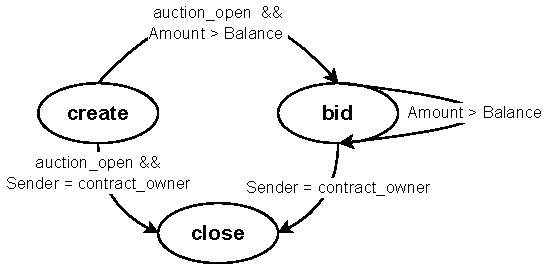
\includegraphics[width=1.1\textwidth]{auction-life-cycle}
    \caption{Auction contract life cycle}
    \label{fig:auction-life-cycle}
\end{figure}


\section{Static Checker}
\label{sec:static-checker-we}
We verify the contract against its specifications in the contract
module by symbolic execution. Symbolic execution involves calculating
a symbolic stack at each transition from one Michelson instruction to
the next. The symbolic interpreter is fully typed and rejects
ill-typed Michelson programs, provided the ill-typed part is reachable
from the default entry point.  The initial stack is derived from the
input term for each the entry point. To maintain symbolic values as
concrete as possible, some instructions may be deemed unreachable or
only reachable under specific conditions. This process yields, for
each entry point, a set of final symbolic stacks accompanied by a path
condition indicating when this final state is reachable. A state is
discarded from the final state space if the path condition is not
satisfiable, indicating that the path is unreachable. Additionally,
for each \FAILWITH\ instruction, we obtain a symbolic value for the
reported message and a path condition indicating the reachability of
this instruction. We employ the SMT solver Z3  to assess the
satisfiability of a path condition and to check smart contract
properies specified by pre- and post conditions.

%The architecture of the static checker is illustrated in Figure~\ref{fig:architecture-of-static-checker}. 
The system comprises three phases. The first phase is user specification, where users
provide the Michelson code of the contract and define the properties
that the smart contract should satisfy. Subsequently, the symbolic
interpreter is run on the code with the provided input term.  The
path conditions are then fed into a Z3 converter, which transforms
symbolic terms into Z3 formulas. Concurrently, the property
specification, specifically pre- and post conditions, also undergoes
conversion to Z3 formulas. The results of the symbolic execution and
Z3 formulas are then input into the static checker, which verifies
whether these properties hold for the smart contract
implementation. This constitutes the verification phase. 

\subsection{User specification}
\label{sec:user-specification}

In the user specification phase, users compose the specification in
our domain-specific language using the syntax outlined in
Section~\ref{sec:domain-specific-language}. Michelson code, whether
composed by users, obtained from the Tezos blockchain, or compiled
from higher-level languages, can be seamlessly used within our
framework. The specification is subsequently parsed into an Abstract
Syntax Tree (AST) in OCaml. The code and the input term are then
input to the symbolic interpreter. In the next phase, the pre- and
post-predicates are transformed into Z3 formulas by the Z3 converter.

\subsection{Michelson interpreter and Z3 converter}
\label{sec:mich-interpr-z3}
The symbolic interpreter implements the execution model described in
Section~\ref{sec:symbolic-execution-model}. When provided with a
concrete input, the interpreter produces a concrete value. In the
presence of symbolic input, the result comprises a set of symbolic
states represented as terms in OCaml. As Michelson's infrastructure is
implemented in OCaml, the conversion of Michelson types or terms to
their OCaml counterparts is straightforward. Each state contains the
output stack, which has only one element consisting of an operation
list and storage, along with the path conditions represented as
predicates in conjunctive normal form. This output is then fed into
the Z3 converter, which handles two different types of terms:
assertion terms from the AST representing the pre- and post-condition
specifications, and terms resulting from the interpreter. We utilize
the Z3 library in OCaml to construct this converter. Some adjustments
are necessary to convert these terms into Z3 formulas. For example, as
there is no natural number type (\TNAT) in Z3, it is injected to Z3's
integer type with a constraint asserting that the value is greater
than or equal to zero. Several constants, such as \CAMOUNT, \CBALANCE,
\CSENDER\ as well as cryptographic functions, such as \FSHA,
\FHASHKEY\ are predefined in the environment that works for any smart
contract specifications. 

% \paragraph{Dealing with loop formalization}
% \label{sec:dealing-with-loop}
Our execution model formalizes loops symbolically using the \FOLD\ and
\FMAP\ functions (see
Section~\ref{sec:symbolic-execution-model}). This approach has the
advantage of allowing us to convert these loops into formulas
compatible with certain SMT solvers, such as Z3, which support these
functions. Specifically, Z3 provides \lstinline/seq.map fn s/, a map
function on sequence \lstinline/s/, and
\lstinline/(seq.foldl fn b s)/, a fold function with an initial value \lstinline/b/ on sequence
\lstinline/s/. These functions are supported for checking assertions
that contain them. Therefore, we can directly convert the symbolic
results of loops into formulas in Z3. 
\subsection{Static checker}
\label{sec:static-checker}
The static checker now performs the verification process by employing symbolic execution against the property specification in the DSL. It utilizes the results from the previous phases, including symbolic execution, Z3 formulas representing pre and post conditions, and path conditions. 

We first build the input state from the input term and run the
symbolic interpreter on the input stack with the provided code to
generate all symbolic execution states. Symbolic execution ensures
that all states are reachable from the initial state, as any
unreachable states are discarded from the final states as their path
conditions are unsatisfiable. Using the output term and the pre-
and post-conditions converted by the Z3 conveter, the tool then
performs different checks. The static checker offers three distinct
features: output check, fail condition, and property check. 

\subsubsection{Output check}
\label{sec:output-check}
The first check is the output check, where the checker verifies
whether the output term matches. The final state contains a stack
with only one element as \Stack\ \STACKCONCAT\ \EMPTYSTACK. There are
two different forms of the final state. In the case where the code is
given as incomplete smart contract code, the element \Stack\ contains
just a normal term and its corresponding type as (\Term,
\TY). However, in the case of a complete smart contract code, it has
the form (\PAIR\ \VOPERATIONLIST\ \VSTORAGE, \TPAIR\ (\TOPERATIONLIST)
\TYS) \STACKCONCAT\ \EMPTYSTACK, where \VSTORAGE\ is the term
representing the storage and \VOPERATIONLIST\ repesents a operation
list. Given an output term $ \tau$, the checker scans all the reachable final
states, which do not contain a failwith stack and checks whether the
output term matches. In the former case, it matches $ \tau$  with
the term \Term. In the latter case, it essentially matches with the
corresponding part \VSTORAGE\ in the final states resulting from the
symbolic interpreter. When the input term is a concrete value, the
result from the interpreter is also concrete, and then the checker can
be used to verify if the output aligns with the expectations
specified in the output field. 

Listing~\ref{lst:sub-contract-specification} contains an example of an
incomplete smart contract code. The specification states that the
output of the code must be a stack that contains only one element of
type \TINT\, symbolically represented as a variable \VZ\ of type
\TINT.  In this example, there are two final states, the first one
being a failwith state recording the failwith condition when the first
element of the pair is less than the second element. The failwith
state contains the message \lstinline|'Unexpected Pair'|, which
describes the reason for the failure. The second state is a reachable
state that contains, in the top element, an integer value, which is
the substract of the two elements of the pair. The output check succeeds for
this example as expected. However, this test could fail if, for
example, the output term is incorrectly specified as a variable of
a type that does not match with the actual result. If the input
term is concrete, for instance, a pair of numbers as in
\lstinline|Pair 5 3|, then the expected output should be the number
\lstinline|2|. To check this,  the output term may be specified as
a concrete value.

The second example in Listing \ref{lst:auction-contract-specification}
is the specification for a smart contract code. The output term
represents the updated storage after executing the code. There are
several final states resulting from the symbolic execution. The
failwith state is ignored for the output check, and all other
reachable states are matched with the output term. The output check
succeeds for this example.

\subsubsection{Fail condition}
\label{sec:fail-condition}
A Michelson contract can fail due to a programmer-induced condition
caused by the instruction \FAILWITH. It terminates contract execution
with an error message reported back to the caller. This error message
includes the top value on the stack. These failures are important in
smart contract programming to guarantee that a smart contract call
should not be successful under specific circumstances. Smart contract
calls are expected to fail due to malicious behavior, such as an
unauthorized caller or invalid arguments passed along the call. For
example, the auction contract should not be closed by someone who is
not the owner of the contract, and the bidding should not succeed if
the bid is not strictly higher than the current highest bid. Several
smart contract standards, such as
\cite{erc, fa}, require the contract to fail
with specific messages under certain conditions. Therefore, it is
essential to check the fail conditions of a contract.  

The static checker provides a feature to generate all fail conditions
implemented in a smart contract code. The tool searches for all
failwith states, resulting from an execution terminated by the
\FAILWITH\ instruction, from the final state space, collects the path
conditions and the recorded message. The result returned to users
includes the fail condition together with the message. For example,
for the specification in Listing \ref{lst:sub-contract-specification},
the fail condition is recorded as
\lstinline/(x < y): 'Unexpected Pair'/.  

The ability to generate fail conditions is a potent feature of our
static checker, particularly in verifying access control properties
across various smart contracts. Specifically, in numerous smart
contract configurations, certain entrypoints are designated for
invocation only by authorized entities, for instance, by the contract
owner. Consequently, these entrypoints must result in failure if the
callers lack the necessary authorization. This crucial access control
property is verified by examining the fail conditions of a smart
contract, ensuring that unauthorized callers trigger the intended
failures in the system. 

The auction contract exhibits several fail conditions. For the
entrypoint \lstinline/bid/, the fail condition is as shown in
Listing~\ref{lst:fail-condition-auction-contract-bid} and for the
\lstinline/close/ entrypoint, it is recorded in
Listing~\ref{lst:fail-condition-auction-contract-close}. For the
\lstinline/bid/ entrypoint, there are three fail conditions.  (1) If
the auction is closed, (2) if the auction is open, but the amount less
than or equal to the balance, (3) if the auction is open, the amount
is greater than the balance, but the highest bidder's address is
invalid. The last failure can happen because there are valid Michelson
addresses, which are not associated with any real account on the Tezos
blockchain, or the parameter's type is not correct: the transfer can
only succeed if the address is associated with an account and the
parameter supplied matches with the parameter expected by the Tezos
blockchain. Bidding returns the previous highest bid as part of the
transaction where the highest bidder is stored as a value of type
address. However, to receive a token transfer, this address must be
cast (by the Michelson implementation of the contract) to an implicit
contract of Michelson type (\TCONTRACT\ \TUNIT). This cast is
unavoidable, as a value of contract type cannot be stored.  However,
the cast may fail for the reasons just discussed, and its failure
leads to an error condition that is reported with a \FAILWITH\
instruction in the implementation. The \lstinline/close/ entrypoint has
similar fail conditions when the auction is closed or the owner's
address is cannot be cast. The other fail condition occurs when the
auction is open, but the sender who calls this entrypoint is not the
owner of the contract, which was stored in the contract owner part.

\begin{lstlisting}[float=tp,captionpos=b,caption={Fail condition for auction contract bid entrypoint },label={lst:fail-condition-auction-contract-bid},numbers=left]
1. not (auction_open = true): 'Already closed'
2. (auction_open = true) && not (Amount > pre_Balance):
   'Not higher than the current highest bid'
3. (auction_open = true) && (Amount > pre_Balance) && 
   get_contract (unit, highest_bidder) = None:
   'Invalid highest bidder address' 
\end{lstlisting}

\begin{lstlisting}[float=tp,captionpos=b,caption={Fail condition for auction contract close entrypoint},label={lst:fail-condition-auction-contract-close},numbers=left]
1. not (auction_open = true): 'Already closed'
2. (auction_open = true) && not (Sender = contract_owner): 
    'Not the owner'
3. (auction_open = true) && (Sender = contract_owner) &&
   get_contract (unit, contract_owner) = None:
  'Invalid contract owner address'
\end{lstlisting}

In this implementation of the auction contract, the failures are
recorded as expected. The contract is designed to fail when the
auction is closed, the bid is not greater than the old highest bid, or
the caller is not the contract owner when attempting to close the
contract as transferring the contract balance to their account as a
part of the action. 

\subsubsection{Property check}
\label{sec:property-check}

The static checker enables users to verify smart contract properties
by providing pre- and post-condition specifications. A property is
specified with the clause:  \lstinline/pre-condition := &&/
$\Phi_{i}$ followed by \lstinline/post-condition := &&/ $\Psi_{j}$. This
specification asserts that if all preconditions $\Phi_{i}$ hold before
smart contract execution, then all $\Psi_{j}$ must hold after
successful (i.e., without failure) termination. To verify this
property, we explore all the paths $\Pi$ 
with the path condition $\Theta$ such that ($\bigwedge \Phi_{i}$
$\land$ $\Theta$) is satisfiable. We then check that for every path
$\Pi$, $\neg$ ($\bigwedge \Phi_{i}$ $\land$ $\Theta$ $\rightarrow \bigwedge \Psi_{j}$) is unsatisfiable in the context given by the input for the entry point
and its corresponding final state.

Consider the specification of the sub contract in Listing
\ref{lst:sub-contract-specification}. In this context, the two
variables \lstinline/x/ and \lstinline/y/ are integers. The results of
the symbolic execution are either a failwith state with the path
condition \lstinline/x/$<$\lstinline/y/,  or a state in which the
final stack has only one element, which is a symbolic variable
\lstinline/sbvar/ of type integer, with the path condition stating
that the variable \lstinline/x/ is greater than or equal to
\lstinline/y/ and the symbolic variable \lstinline/sbvar/ is equal to
the substract of \lstinline/x/ and \lstinline/y/.  For this specification,
the failwith branch is discarded because the precondition is not
satisfy with the	 path condition, and then \lstinline/z/ is matched to
the symbolic variable \lstinline/sbvar/ in the other branch. In this
example, the checker then verifies that $\neg$ ((\lstinline/x/ >= y) $\land$ (\lstinline/z/
= \lstinline/x/ - \lstinline/y/) $\rightarrow$ (\lstinline/z/ = \lstinline/x/ - \lstinline/y/) $\land$ (\lstinline/z/ >= 0)) is unsatisfiable.

\subsubsection{Life-cycle check}
\label{sec:life-cycle-check}
An entrypoint relation can be defined as \lstinline/(%a -> %b) with cd/, indicating that after invoking the entrypoint \lstinline/%a/, it is permissible to call the entrypoint \lstinline/%b/ if the condition \lstinline/cd/ is satisfied. The presence of the keyword \lstinline/not/ at the beginning signals an impossibility. Note that \lstinline/with cd/ may be omitted when no condition is needed.

Let $S_a$ represent the set of all reachable states resulting from the execution of the call to the entrypoint \lstinline/%a/. Each $s_{i}$ in $S_a$ is associated with a path condition $\Theta_i$ and is represented as a stack containing a single element—a pair consisting of an operation list ($\VOPERATIONLIST_i$) and the storage $\VSTORAGE_i$. For each $s_{i}$, symbolic execution is performed on the entrypoint \lstinline/%b/ using input as a pair of the parameter and the storage $\VSTORAGE_i$, constrained by $\Theta_i$ and the condition \lstinline/cd/. In the execution state space, a state $s_{j}$ with the path condition $\Theta_j$ is considered reachable if ($\Theta_i$ $\land$ \lstinline/cd/ $\land$ $\Theta_j$) is satisfiable, and $\neg$ ($\Theta_i$ $\land$ \lstinline/cd/ $\rightarrow$ $\Theta_j$) is unsatisfiable. Let $S_b$ denote the set of these reachable states. If $S_b$ is empty or contains only failwith states, then it is impossible to invoke the entrypoint \lstinline/%b/ from the state $s_{i}$. Otherwise, it is considered a success. Let $R$ be the set containing all such states $s_{i}$ in $S_a$ where it is successful to call the entrypoint \lstinline/%b/ with the condition \lstinline/cd/. If $R$ is non-empty, then \lstinline/(%a -> %b) with cd/ holds. Otherwise, it is false, signifying \lstinline/not (%a  -> %b) with cd/.

\section{Case Studies}
\label{sec:case-stud-subs}

This section reports two case studies that we conducted with the
implemented system. Both case studies are real contracts deployed on
the Tezos blockchain and are taken from the realm of financial
applications. 

\subsection{USDtz}
\label{sec:usdtz}

In a blockchain ecosystem, tokens represent digital assets that can be
transferred between accounts. These tokens are securely stored and
verified within the blockchain network. There are various types of
tokens, including native tokens (cryptocurrencies) like Bitcoin,
Ether, Tezos, and others. Additionally, tokens can be created as
overlays through smart contracts on an existing blockchain. Two common
categories are: (1) Fungible Tokens (FT), which are interchangeable
and (2) Non-Fungible Tokens (NFTs), which represent unique digital
assets, and each unit is distinct. Stablecoins, falling under fungible
tokens, are designed to maintain a stable value by tracking the value
of a fiat currency like USD or EUR.

While designers can create tokens that behave in any way they want, it
is advisable to implement tokens that adhere to established standards.
This adherence guarantees interoperability and compatibility across
different platforms. A token standard defines a set of rules and an
interface that smart contracts must follow to ensure compatibility
with decentralized exchanges, wallets, and other tools within the
ecosystem. For example, ERC-20 \cite{erc} is a token standard used in Ethereum \cite{eth-whitepaper}.  


The Tezos blockchain has its own set of standards known as Financial
Applications (FA). Two notable standards are: (1) FA 1.2 \cite{fa}, designed for
fungible tokens, and (2) FA 2 \cite{fas}, a more versatile standard accommodating
both fungible and non-fungible tokens (NFTs). The standard outlines a
smart contract that functions as a ledger, associating identities with
balances. This ledger is designed to facilitate token transfer
operations and enable approvals for spending tokens from other
accounts. Any contract aiming to implement the standard must
incorporate the functions specified in
Listing~\ref{lst:fa12-interface} such as token transfer (transactions
between users), approval (allowing one user to send tokens from
another user's address),  allowance (browsing the amount of tokens
available for an account to sending from another address), user
balance (checking the balance of a user), and current supply (checking
the total supply of tokens across all addresses), where
\lstinline/view a r = pair a (contract r)/ implies an view entrypoint.
A view is an entrypoint that takes an
argument of type \lstinline/a/ and a contract to callback that receives in a value
of type \lstinline/r/. The callback in this case will be another
contract address. Further elaboration on the details of FA 1.2 can be
found in \cite{fatzip}, and we will delve into
these functions in subsequent 
sections.

\begin{lstlisting}[float=tp,captionpos=b,caption={FA 1.2 interface},label={lst:fa12-interface},numbers=left]
(address :from, (address :to, nat :value))    %transfer
(address :spender, nat :value)                %approve
(view (address :owner, address :spender) nat) %getAllowance
(view (address :owner) nat)                   %getBalance
(view unit nat)                               %getTotalSupply
\end{lstlisting}

In this section, we verify USDtz \cite{usdtzimplemetation}, an
implementation of the FA 1.2 standard. Our goal is to ensure that the
implementation aligns with the standard, verifying its
correctness. USDtz is a stablecoin and one of the first and
longest-running coins on the Tezos blockchain, launched in September
2020. The smart contract is located at the address
\texttt{KT1LN4LPSqTMS7Sd2CJw4bbDGRkMv2t68Fy9}, and the code can be
found on the Tezos blockchain \cite{tzstatsusdtz}. USDtz adheres to
the FA token standard, and the initial deployment of the USDtz smart
contract follows the FA 1.2 standard. 
The implementation consists of approximately 1000 instructions. It
contains all five entrypoints required in the FA 1.2 interface and
four additional ones.  We will verify each entrypoint of this smart
contract. First, we examine how the approvable ledger is implemented
in the USDtz smart contract. The ledger is a substantial map that
links user addresses to a pair consisting of their balance and a map
associating addresses with the amount of tokens allowed to be
transferred from that user's
account. Listing~\ref{lst:storage-udstz-contract} shows the storage type of the
USDtz smart contract.  

\begin{lstlisting}[float=tp,captionpos=b,caption={Storage of the USDtz smart contract},label={lst:storage-udstz-contract}]
(pair
  (big_map %ledger
    (address :user)
    (pair (nat :balance)
          (map :approvals (address :spender) (nat :value))))
  (pair (address %admin)
        (pair (bool %paused) (nat %totalSupply))))
\end{lstlisting}


\subsubsection{transfer}
As illustrated in Listing \ref{lst:fa12-interface}, the
\lstinline/transfer/ entrypoint credits the account associated with
the address provided in the \lstinline/to/ parameter, while debiting
the account corresponding to the \lstinline/from/ parameter with the
specified \lstinline/value/ amount. The FA 1.2 standard mandates that
this call must fail under the following two conditions: (1) In the
event of insufficient balance, this entrypoint MUST fail with the
error \lstinline/NotEnoughBalance/, indicating insufficient funds in
the sender's account to execute the transfer. (2) If the sender's
account has no permission to withdraw the \lstinline/value/ amount of
funds, the call will fail with the \lstinline/NotEnoughAllowance/
error, which also contains the same pair message as the first failure
scenario. To verify these requirements, we utilize the failwith
condition feature of the tool and examine the returned results, as
outlined in Listing~\ref{lst:transfer-udstz-contract}\footnote{There may be some duplicates of the same failwith condition due to the branching of the symbolic interpreter. The results here are shortened. We are working on filtering them in the tool.}.
\begin{lstlisting}[float,captionpos=b,caption={Fail conditions for the \lstinline/transfer/ entrypoint},label={lst:transfer-udstz-contract},numbers=left]
1. (paused = true): 'TokenOperationsArePaused'
2. not (paused = true) 
   && get_big_map (from, ledger) = None : 'NotEnoughBalance'
3. not (paused = true) 
   && get_big_map (from, ledger) = Some sbvar 
   && sbvar = Pair sbvar1 sbvar2 
   && not (sbvar1 >= value) : 'NotEnoughBalance'
4. not (paused = true) 
   && get_big_map (from, ledger) = Some sbvar 
   && sbvar = Pair sbvar1 sbvar2 
   && get_map (Sender, sbvar2) = Some sbvar3 
   && sbvar1 >= value 
   && not (sbvar3 >= value): 'NotEnoughAllowance'
\end{lstlisting}
The fundamental property that this entrypoint should satisfy is the decrement of the allowance of the sender's account by the \lstinline/value/ that has been sent as Listing \ref{lst:specification-transfer}.
\begin{lstlisting}[float,captionpos=b,caption={Specification of the \lstinline/transfer/ entrypoint},label={lst:specification-transfer},numbers=left]
mcontract usdtz = spec 
 storage :=  Pair (ledger: big_map address 
  (pair nat (map address nat))) 
  (Pair (admin: address) 
          (Pair (paused: bool) (total_supply: nat)))
 entrypoint %transfer
   parameter := Pair (from: address)
         (Pair (to: address) (value: nat))
   pre-condition := not (paused  = true)
     && get_big_map (from, ledger) = 
       Some (v: pair nat (map address nat))
     && v = Pair (n: nat) (m: map address nat)
     && get_map (Sender, m) = Some (k: nat) 
     && (n >= value) && (k >= value)
   post-condition := get_big_map (from, post_ledger) = 
     Some (post_v:  pair nat (map address nat))
     && post_v = Pair (post_n: nat) (post_m: map address nat) 
     && get_map (Sender, post_m) = Some (post_k: nat) 
     && (post_n = n - value) && (post_k = k - value)
\end{lstlisting}

\subsubsection{approve}
\label{sec:approve}

The \texttt{approve} entrypoint takes a spender address and an
amount. It grants the spender the right to transfer that amount from
the owner's account.

The crucial property to ensure the correctness of the \texttt{approve}
entrypoint is that changing the allowance value from a non-zero value
to another non-zero value is forbidden to prevent a corresponding
attack vector \cite{attack-vector}. The basic idea of this attack is
that when a non-zero value update is allowed, the \lstinline/spender/
can attempt to spend the entire allowance before the new amount is
updated and then spend again with the new value, resulting in a larger
amount than actually allowed. Hence, the contract call must fail when
both the parameter \lstinline/value/ is non-zero and the allowance of
\lstinline/spender/ is also non-zero. We verify this property by
generating a fail condition, so that a non-zero value update is
recorded as a fail condition, as shown in
Listing~\ref{lst:approve-udstz-contract}. This condition indicates
that the implementation ensures the non-zero value update prevention. 
\begin{lstlisting}[float=tp,captionpos=b,caption={Fail conditions for the \lstinline/approve/ entrypoint},label={lst:approve-udstz-contract},numbers=left]
1. (paused = true): 'TokenOperationsArePaused'
2. not (paused = true) 
   && get_big_map (Sender, ledger) = Some sbvar 
   && sbvar = Pair sbvar1 sbvar2 
   && get_map (spender, sbvar2) = Some sbvar3 
   && not (value = 0) 
   && not (sbvar3 = 0): 'UnsafeAllowanceChange'
\end{lstlisting}
If the update is allowed, then the updated value needs to be recorded
correctly in the storage. This property can be divided into two
subproperties, which can be checked separately. Property 1: if the
parameter \lstinline/value/ is zero, then the 
corresponding allowance value of the \lstinline/spender/ from the
owner (which is \SENDER\ in this call) should be zero. This
subproperty is specified as shown in
Listing~\ref{lst:specification-approve-1}. Property 2: if
\lstinline/value/ is non-zero and the allowance of the \lstinline/spender/ is zero, then the \lstinline/value/ should be recorded in the storage after the call. We specify this property using pre- and post-conditions, as illustrated in Listing~\ref{lst:specification-approve-2}.

\begin{lstlisting}[float=tp,captionpos=b,caption={Specification of the \lstinline/approve/ entrypoint (Property 1)},label={lst:specification-approve-1},numbers=left]
entrpoint %approve
   parameter := Pair (spender: address) (value: nat)
   pre-condition := not (paused = true)
      && get_big_map (Sender, ledger) = 
        Some (v: pair nat (map address nat))
      && v = Pair (n: nat) (m: map address nat) 
      && get_map (spender, m) = Some (k: nat) 
      && not (k = 0) && (value = 0)
   post-condition := get_big_map (Sender, post_ledger) = 
        Some (post_v:  (pair nat (map address nat))
      && post_v = Pair (post_n: nat) (post_m: map address nat) 
      && get_map (spender, post_m) = Some (post_k: nat) 
      && (post_k = 0) ;
\end{lstlisting}
\begin{lstlisting}[float=tp,captionpos=b,caption={Specification of the \lstinline/approve/ entrypoint (Property 2)},label={lst:specification-approve-2},numbers=left]
   pre-condition := not (paused = true) 
      && get_big_map (Sender, ledger) = 
        Some (v: option (pair nat (map address nat))) 
      && v = Pair (n: nat) (m: map address nat) 
      && get_map (spender, m) = Some (k: nat) 
      && (k = 0) && not (value = 0)
   post-condition := get_big_map (Sender, post_ledger) = 
        Some (post_v: option (pair nat (map address nat))) 
      && post_v = Pair (post_n: nat) (post_m: map address nat) 
      && get_map (spender, post_m) = Some (post_k: nat) 
      && (post_k = value) ;
\end{lstlisting}

\subsubsection{getAllowance, getBalance,  getTotalSupply}
\label{sec:getall-getb-gett}

These entrypoints are view entrypoints. View entrypoints are functions
that retrieve information from the storage but do not change the state
of the smart contract. As indicated in
Listing~\ref{lst:fa12-interface}, the results of these entrypoints are
natural numbers, which are sent back to specific addresses, which must
be tied to smart contracts with entrypoints that have a parameter type
of \lstinline/nat/. The implementation of a view entrypoint must
return the \lstinline/TRANSFER_TOKENS/ operation targeting the
contract passed as an argument with precise information, namely the
amount of tokens \lstinline/spender/ is allowed to spend from the
\lstinline/owner/ for the \lstinline/getAllowance/ entrypoint, the
balance of the owner \lstinline/owner/ for the \lstinline/getBalance/
entrypoint, and the total supply for the \lstinline/getTotalSupply/
entrypoint. Additionally, the transaction must transfer to the
callback contract with an amount equal to \AMOUNT. In other words, all
the Tezos-tokens passed to a view entrypoint are forwarded to the
callback contract. Another important property is that there should be
no modification in the ledger when these entrypoints are called. 

As an example, we demonstrate how to verify the \lstinline/getBalance/
entrypoint,  shown in Listing~\ref{lst:specification-get-balance}. The
other entrypoints \lstinline/getAllowance/ and
\lstinline/getTotalSupply/ can be specified similarly.  There are two
cases to consider: (1) if the \lstinline/owner/ is in the
\lstinline/ledger/ big map and (2) if it is not. For the former case,
lines 5-8 specify that \lstinline/owner/ is in the \lstinline/ledger/
big map, as the \lstinline/get_big_map/ function returns a value
\lstinline/Some value/ of the \TOPTION\ type, and this
\lstinline/value/ is a pair of a natural number \lstinline/k/ and a
map \lstinline/m/. The postcondition guarantees that the storage
remains unchanged, as specified in lines 10-13, and the call returns a
\lstinline/TRANSFER_TOKENS/ operation with the \lstinline/k/ number
and \lstinline/Amount/ to be passed to address \lstinline/c/. The
precondition in lines 16-17 specifies the latter case when the
\lstinline/owner/ does not exist in the big map \lstinline/ledger/; in
this case, the number \lstinline/0/ should be sent, and again, the
storage should remain unchanged. 

\begin{lstlisting}[float=tp,captionpos=b,caption={Specification of the \lstinline/getBalance/ entrypoint},label={lst:specification-get-balance},numbers=left]
entrypoint %getBalance
   parameter := Pair (owner: address) (c: contract nat)
   pre-condition :=  get_big_map (owner, ledger) = 
        Some v: option (pair nat (map address nat)) 
      && v  = Pair (k: nat) (m: (map address nat))
   post-condition := post_ledger = ledger 
      && post_admin = admin 
      && post_paused = paused 
      && post_total_supply = total_supply 
      && post_Balance = pre_Balance 
      && transfer_token (k, Amount, c) ;

   pre-condition :=  get_big_map (owner, ledger) = 
        None option (pair nat (map address nat)) 
   post-condition := post_ledger = ledger 
      && post_admin = admin 
      && post_paused = paused 
      && post_total_supply = total_supply 
      && post_Balance = pre_Balance 
      && transfer_token (0, Amount, c) ;
\end{lstlisting}
\subsubsection{Further entrypoints}
\label{sec:other-entrypoints}

The contract provides five additional entrypoints: \lstinline/mint/ to
mint you own tokens, \lstinline/burn/ to burn existing tokens,
\lstinline/setAdministrator/ and \lstinline/getAdministrator/ to set
up or retrieve the administrator of the smart contract, and
\lstinline/setPause/ to pause the contract. To generate fail
conditions, we detect that \lstinline/transfer/ or \lstinline/approve/
calls fail if the contract is in a paused state. Users or dapps should
be aware of this when interacting with the smart contract. 

The \lstinline/mint/ and \lstinline/burn/ entrypoints affect the total
supply, so they should act consistently with the amount mined or
burned. Obviously, only the administrator is allowed to call these
entrypoints. The same holds for the \lstinline/setPause/ entrypoint.

The administrator plays a crucial role in this contract. Therefore,
for the \lstinline/setAdministrator/ entrypoint, it must be guaranteed
that only the current administrator can call this entrypoint and the
new administrator must match the address passed through the
parameter. Another property to ensure is that, except for this
entrypoint call, any other smart contract call to this contract should
not change the administrator. 

All of the above-mentioned properties are specified and verified in
our model. The results show that these properties are guaranteed,
i.e., that the smart contract code is correct.

\subsection{Kolibri Oracle Contract}
\label{sec:kolibri-oracle-contr}
The potential of smart contracts is constrained by the inability to
access external data sources. To address this limitation, oracles
serve as a crucial link between external sources and the blockchain
network.  Blockchain oracles play a pivotal role in furnishing
external data for smart contracts. Certain essential properties must
be satisfied by an oracle contract, including data approvability. This
case study aims to illustrate the process of specifying and verifying
an oracle contract by the static checker, using the Kolibri oracle
contract as an example.


The Kolibri oracle contract \cite{kolibri},  residing at  address
\texttt{KT1Tj6xknbwjyK5gyfESNR6WESBcP3yX1mmj} \cite{tzstatskolibri}, ensures the accuracy of
external data for the Tezos-based stablecoin Kolibri by leveraging
the Harbinger Price Feed. The contract initiates calls to a Harbinger
Normalizer contract, checks the returned values, normalizes them to
suit the Kolibri system, and subsequently relays them to the
client. The smart contract's parameters and storage details are
outlined in Listing~\ref{lst:kolibri-oracle-contract}. Key attributes
stored by the oracle include:

\begin{itemize}
\item \lstinline/harbingerContractAddress/: the address of the Harbinger Price Feed contract.
 \item    \lstinline/state/: a natural number indicating the current state of the contract: (1) \lstinline/IDLE/ and (2) \lstinline/WAITING_FOR_HARBINGER/.
 \item    \lstinline/clientCallback/: a contract featuring a \TNAT\ entrypoint that stores state when the oracle awaits Harbinger data.
 \item    \lstinline/governorContractAddress/: the address of the governor contract. The governor is the controler of the oracle contract as it is able to update on the contract such as reset the maximu time for data delay.  
 \item    \lstinline/maxDataDelaySec/: the maximum acceptable age of data received from Harbinger, measured in seconds.
\end{itemize}
The oracle contract offers various entrypoints, including:
\begin{itemize}
\item    \lstinline/getXtzUsdPrice/: retrieval, sanity check, and normalization of Harbinger data.
\item    \lstinline/getXtzUsdPrice_callback/: serves as a callback mechanism to receive data from Harbinger.
\item    \lstinline/default/: always intentionally fails to prevent the transfer of XTZ into the contract.
\item    \lstinline/setMaxDataDelaySec/: enables the setting of the maximum acceptable age for data received from Harbinger.
\item    \lstinline/setGovernorContract/: allows the setting of the Governor's address.
\end{itemize}

\begin{lstlisting}[float,captionpos=b,caption={Kolibri oracle contract},label={lst:kolibri-oracle-contract},numbers=left]
parameter
 (or
   (or (unit %default) (contract nat %getXtzUsdRate))
   (or
     (pair string (pair timestamp nat) %getXtzUsdRate_callback)
     (or
       (address %setGovernorContract) 
       (nat %setMaxDataDelaySec)))) ;
storage
 (pair
   (pair (option %clientCallback address) 
         (address %governorContractAddress))
   (pair (address %harbingerContractAddress) 
         (pair (nat %maxDataDelaySec) (int %state)))) ;
\end{lstlisting}

Another critical access control property is the resettable nature of \lstinline/governorContractAddress/ and \lstinline/maxDataDelaySec/. While these parameters are designed to be reset, such actions should exclusively be carried out by the governor. Maintaining this restriction is paramount to prevent loss of control over the contract in the event of unauthorized resets. In practical terms, the entrypoints \lstinline/setGovernorContract/ and \lstinline/setMaxDataDelaySec/ must only be invocable by the governor. Any attempts by unauthorized callers to make these calls should result in failure to ensure the integrity of access control and prevent potential misuse of these critical parameters.

The Kolibri oracle contract maintains a straightforward state machine comprising two states: (1) \lstinline/IDLE/ and (2) \lstinline/WAITING_FOR_HARBINGER/. From the \lstinline/IDLE/ state, the oracle can exclusively transition to the \lstinline/WAITING_FOR_HARBINGER/ state. The \lstinline/getXtzUsdPrice/ entrypoint is permissible only when the oracle is in the \lstinline/IDLE/ state, and invoking this entrypoint transitions the oracle to the \lstinline/WAITING_FOR_HARBINGER/ state. Notably, in the \lstinline/IDLE/ state, the value of \lstinline/clientCallback/ is always set to none. Conversely, from the \lstinline/WAITING_FOR_HARBINGER/ state, the oracle can only transition back to the \lstinline/IDLE/ state. The \lstinline/getXtzUsdPrice_callback/ entrypoint is allowable solely when the oracle is in the \lstinline/WAITING_FOR_HARBINGER/ state, and invoking this entrypoint results in the oracle transitioning to the \lstinline/IDLE/ state. In the \lstinline/WAITING_FOR_HARBINGER/ state, the value of \lstinline/clientCallback/ is always set to some.

Several properties must be verified to ensure the correct functioning of the state machine. The initial property states that \lstinline/getXtzUsdPrice/ can only be invoked when in the \lstinline/IDLE/ state, while conversely, \lstinline/getXtzUsdPrice_callback/ can only be invoked when in the \lstinline/WAITING_FOR_HARBINGER/ state. The validation of this property involves examining the fail conditions of these two entrypoints.

The subsequent property dictates that if \lstinline/getXtzUsdPrice/ is successfully executed, the state must transition to \lstinline/WAITING_FOR_HARBINGER/, and the parameters passed along with the call need to be stored in the \lstinline/clientCallback/ attribute of the storage.

The following property asserts that if \lstinline/getXtzUsdPrice_callback/ is successful, the state should revert to \lstinline/IDLE/, and there must be a transaction transferring the data to the client at the \lstinline/clientCallback/ attribute. 

The final property concerns the entrypoint relation between
\lstinline/getXtzUsdPrice/ and \lstinline/getXtzUsdPrice_callback/ as
depicted in Figure \ref{fig:kolibri-oracle-emtrypoint-relations}. From
the \lstinline/getXtzUsdPrice/ entrypoint, the contract can only be
called with \lstinline/getXtzUsdPrice_callback/ and then
reverted. Invoking the \lstinline/getXtzUsdPrice/ entrypoint after
another call or invoking the \lstinline/getXtzUsdPrice_callback/
entrypoint again is not allowed. 

The specification of  the contract is showned in Listing \ref{lst:kolibri-contract-specification}. Here, we shortened the names of the variables for the storage.
\begin{figure}[tp]
    \centering
    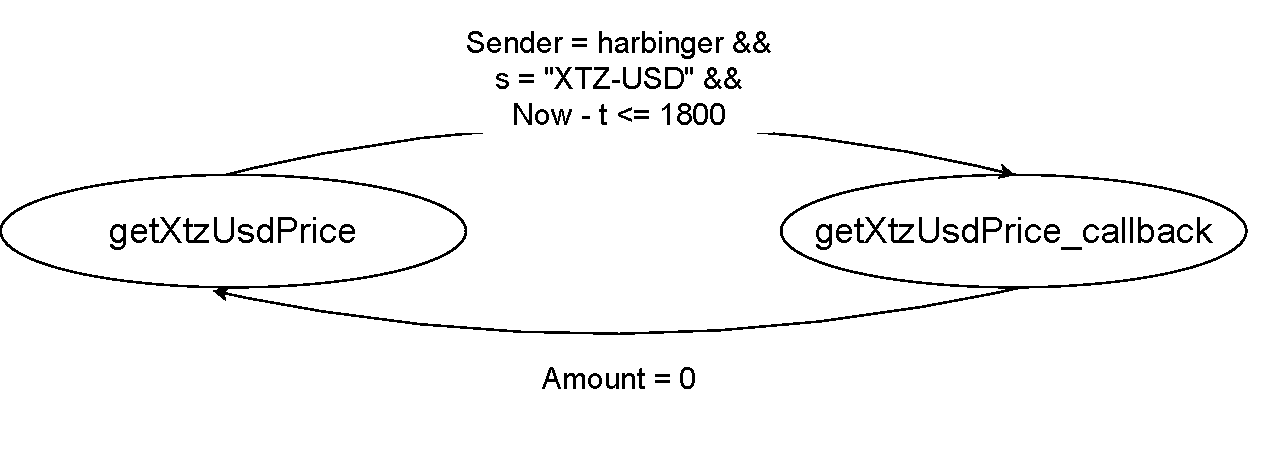
\includegraphics[width=0.8\textwidth]{kolibri}
    \caption{Kolibri oracle entrypoint relations}
    \label{fig:kolibri-oracle-emtrypoint-relations}
\end{figure}

\begin{lstlisting}[float=tp,captionpos=b,caption={Kolibri oracle contract specification},label={lst:kolibri-contract-specification},numbers=left]
mcontract kolibri = spec 
  storage := (Pair (Pair (client: option address) 
     (governor: address))
     (Pair (harbinger: address) 
           (Pair (maxDelay: nat) (state: int))))
  entrypoint %getXtzUsdRate
    code := {...}
    parameter := (ct : contract nat) 
    pre-condition := (Amount = 0) && (state = 0)
    get_contract (pair string (contract pair 
    string (pair timestamp nat)), harbinger) = Some c
    post-condition := state = 1
       && client = Some (b: address) ;
  entrypoint %getXtzUsdRate_callback
    code := {...}
    parameter := Pair (s: string) 
       (Pair (t: timestamp) (n: nat))
    pre-condition :=  state = 1 
       && Sender = harbinger  
       && s = 'XTZ-USD' 
       && Now - t < maxDelay 
       && Now - t >= 0 
       && client = Some a 
       && get_contract (nat, a) = Some c    
    post-condition := state = 0 
       && post_client = None 
       && transfer_token(n, 0, c) ;
  entrypoint %setGovernorContract
    code := {...}
    parameter := (gover : address) 
    pre-condition :=  (Sender = governor)                  
    post-condition := (governor = gover) 
       && (post_maxDelay = maxDelay) 
       && (post_harbinger = harbinger) ;
  entrypoint %setMaxDataDelaySec
    code := {...}
    parameter := (delay: nat)
    pre-condition := (Sender = governor)             
    post-condition := (maxDelay = delay) 
       && (post_client = client) 
       && (post_harbinger = harbinger) ;
  (%getXtzUsdRate -> %getXtzUsdRate_callback) with
     (Sender = harbinger)
     && (s = 'XTZ-USD') 
     && (Now - t >= 0)  
     && (Now - t < maxDelay)  
  | (%getXtzUsdRate_callback  -> %getXtzUsdRate) with 
    (Amount = 0) 
    && get_contract (pair string (contract pair 
    string (pair timestamp nat)), harbinger) = Some c
  | not (%getXtzUsdRate -> %getXtzUsdRate) 
  | not (%getXtzUsdRate_callback -> %getXtzUsdRate_callback)
\end{lstlisting}
When verifying the entrypoint \lstinline/setMaxDataDelaySec/, we noticed an unmatched statement. In \cite{kolibri}, the Kolibri oracle is expected to perform two checks on data returned from Harbinger: (1) was the asset returned "XTZ-USD" and (2) was the asset updated in the last 30 minutes. We ran the fail condition check for both the \lstinline/setMaxDataDelaySec/ and \lstinline/getXtzUsdPrice_callback/ entrypoints as shown in Listing \ref{lst:setXtzUsdPrice_callback} and \ref{lst:setMaxDataDelaySec}. Upon examining the failwith conditions, we detected that there is no failwith if the data is more than 30 minutes (equal to 1800 seconds). We can add the predicate \lstinline/maxDelay <= 1800/ in the post condition of the entrypoint \lstinline/setMaxDataDelaySec/, but then the pre and post condition test fails. This means there is no constraint that the data is less than 30 minutes. This constraint is possibly set up by the governor and specified in the \lstinline/MaxDataDelaySec/ field. However, users calling this contract should be aware that it is possible for the governor to set any value (>=0) as desired. This could lead to providing out-of-date rates.
\begin{lstlisting}[float=tp,captionpos=b,caption={Failwith condition for the entrypoint setXtzUsdPrice\_callback},label={lst:setXtzUsdPrice_callback},numbers=left]
1. not (state = 1): 12
2. (state = 1) && not (Sender = harbinger): 3
3. (state = 1) &&  (Sender = harbinger) 
&& not ('XTZUSD' = s): 14
4. (state = 1) &&  (Sender = harbinger) && ('XTZUSD' = s)
&& (Now - t >= 0) && not (Now - t < maxDelay): 17
5. (state = 1) &&  (Sender = harbinger) && ('XTZUSD' = s)
&& not (Now - t >= 0): Unit
6. (state = 1) &&  (Sender = harbinger) && ('XTZUSD' = s)
&& (Now - t >= 0) && (Now - t < maxDelay) 
&& (client = Some sbvar) 
&& get_contract (Nat, sbvar) = None: Unit
7. (state = 1) &&  (Sender = harbinger) && ('XTZUSD' = s)
&& (Now - t >= 0) && (Now - t < maxDelay) 
&& (client = None): Unit
\end{lstlisting}

\begin{lstlisting}[float=tp,captionpos=b,caption={Failwith condition for the entrypoint setMaxDataDelaySec},label={lst:setMaxDataDelaySec},numbers=left]
not (Sender = governor): 4
\end{lstlisting}
\section{Symbolic Execution Model}
\label{sec:symbolic-execution-model}

We already learned about Michelson, the low-level smart contract
language for the Tezos blockchain, and its stack-based nature in
Section~\ref{sec:background}.  Here we consider the changes needed for
symbolic execution of Michelson programs.

\subsection{System Model}
\label{sec:system-model}

Our symbolic model of a program state is a stack in which each element
is a symbolic value, i.e., a pair consisting
of term and its corresponding type. Terms are defined in
Figure~\ref{fig:term}. Thus we write a stack as \STACK\ = (\TermOne,
\TYF) \STACKCONCAT\ (\TermTwo, \TYS) \STACKCONCAT\ \DOT\ \STACKCONCAT\ 
\EMPTYSTACK\ where \ensuremath{[\ ]} stands for the empty stack and
\ensuremath{hd :: tl} denotes a stack with the top element as
\ensuremath{hd} and the remaining stack as \ensuremath{tl}. 
A selection of types is shown in Figure~\ref{fig:type}.


A Michelson program is a sequence of instructions executed in a
sequential manner. Each instruction takes, as input, the stack
produced by the preceding instruction and modifies it for the
subsequent one. Let \INSTRUCTION\ = \InstructionOne; \InstructionTwo;
\DOT\  \InstructionN\ represent a sequence of instructions.

During symbolic execution,  the system state evolves considering all
values admitted by the constraints on symbolic values. Unless the
input values are sufficiently known, symbolic execution may split the
state, and both constraints and branching conditions are recorded as
predicates. Let \PREDICATE\ be a path predicate that is extended at
each conditional and expressed in conjunctive form, capturing the
branching conditions and constraints encountered during the symbolic
execution process. 
\begin{definition}
A symbolic execution state is represented by a tuple \STATE\ =
[\INSTRUCTION, \STACK, \PREDICATE].
A symbolic system configuration, \SYSTEM\ = \{\STATEONE, \STATETWO,
\DOT, \STATEN \}, is a set of  states.
\end{definition}

The smart contract program takes a stack as input, consisting of a
single pair where the first element is an input value referred to as
parameter denoted as \VPAR\ and the second element represents the
content of the storage space denoted as \VSTORAGE. The program
produces a stack as output, which is a single pair. The first element
of this pair is the list of internal operations that the program
intends to emit (\VOPERATIONLIST), and the second element is the new
contents of the storage space.  We define the initial stack as
\SINIT\   = (\KPAIR\ \VPAR\ \VSTORAGE, \TPAIR\ \TYF\ \TYS)
\STACKCONCAT\ \EMPTYSTACK, where \VPAR\ and \VSTORAGE\ denote terms
representing the parameter and the storage, and \TYF\ and \TYS\ are
their corresponding types. Similarly, a final stack has the form
\SFINAL\   = (\PAIR\ \VOPERATIONLIST\ \VSTORAGE, \TPAIR\
(\TOPERATIONLIST) \TYS) \STACKCONCAT\ \EMPTYSTACK, where
\VOPERATIONLIST\ repesents a operation list.

The initial configuration is \SYSTEMINIT\ = \{[\INSTRUCTION, \SINIT, \TRUE] \}. 

\subsection{Rules}
Each instruction is defined by a rule on a system configuration. There
are several kinds of transitions:
\begin{enumerate}
% \item \ExprTrans\ single-step evaluation of an expression in a system state,
\item \StateTrans\ internal transitions of a state, which is
  non-deterministic  as shown for loop instructions, such as \LOOP\
  and \LOOPLEFT, 
\item \SystemTrans\ symbolic system transitions.
\end{enumerate}

A system transition picks any state and replaces it by all distinct states that
are reachable by internal transitions. It exploits the nondeterminism
of the \StateTrans\ relation.
\begin{mathpar}
  \inferrule[]
  { \STATE\ \StateTrans \STATEONE, \dots, \STATE\ \StateTrans \STATEN
  }{
  \{\STATE\} \cup \SYSTEM \SystemTrans \{ \STATEONE, \dots, \STATEN \}
  \cup \SYSTEM}  
\end{mathpar}
In general, symbolic execution may generate unreachable
states. A state is unreachable if its predicate \PREDICATE\ is  not
satisfiable. Hence, we have a rule that drops unreachable states.
\begin{mathpar}
\inferrule[]
  { \UNSAT\ \PREDICATE
  }{
  \{[\INSTRUCTION, \STACK, \PREDICATE]\} \cup \SYSTEM \SystemTrans \SYSTEM}
\end{mathpar}
The working of the symbolic interpreter may also be understood as a
graph with symbolic states as nodes and internal transitions as
edges. Such a representation makes it easier to perform multi-step
subtransitions as they are required for some operations.

Michelson instructions are categorized based on their functions. The
categories include control structures, stack manipulation, arithmetic
operations, boolean operations, cryptographic operations, and
operations on data structures. In our model, we classify them as
one-step, multi-step, blockchain, cryptographic, branch, and loop
instructions. This categorization reflects how these instructions are
handled within our specific model.

\subsubsection{One-step Instructions}
\label{sec:one-step-instr}
One-step instructions have a localized effect, modifying the system
state directly without branching a new state, and their execution is
modeled with a single rule.
% The ABS rule exemplifies such an
% instruction, operating on the first element of the stack. This element
% must be of type int, and the instruction returns the absolute value of
% its argument as a natural number. To this end, the rule creates a
% fresh variable, \X, and defines its value by a suitable predicate.
% %ABS
% \begin{mathpar}
% \inferrule[ABS]
%   { \X\ \FRESH
%   }
%   {
%     [(\ABS; \INSTRUCTION), (\StackOne, \TINT) \STACKCONCAT \STACK,
%     \PREDICATE]
%     \StateTrans \\
%     [\INSTRUCTION, (\X, \TNAT) \STACKCONCAT \STACK,
%     \PREDICATE\ \wedge\ (\StackOne\ \GE\ \ZERO\ \Rightarrow\ \X\ =
%     \StackOne) \wedge\ (\StackOne\ \LT\ \ZERO\ \Rightarrow\ \X\ = \MINUS\ \StackOne)]
%  }
% \end{mathpar}

For example, the \COMPARE\ instruction for natural numbers compares
the first two elements of the stack, both having a natural number
type. It returns a result of either -1, 0, or 1 based on the
comparison of their values. 
% COMPARE
\begin{mathpar}
\inferrule[COMPARE]
  { \X\ \FRESH
  }
  {
    [(\COMPARE ; \INSTRUCTION), (\StackOne, \TNAT) \STACKCONCAT (\StackTwo, \TNAT)
    \STACKCONCAT \STACK, \PREDICATE ]
    \SystemTrans \\
    [\INSTRUCTION, (\X, \TINT) \STACKCONCAT \STACK, \PREDICATE
    \wedge\ (\StackOne\ \GT\ \StackTwo\ \Leftrightarrow\ \X\ \EQ\ \ONE)
    \wedge\ (\StackOne\ \EQ\ \StackTwo\ \Leftrightarrow\ \X\ \EQ\ \ZERO) 
    \wedge\ (\StackOne\ \LT\ \StackTwo\ \Leftrightarrow\ \X\ \EQ\ \MINUS \ONE)]
    }
\end{mathpar}
\subsubsection{Multi-step Instructions}
Multi-step instructions involve the execution of a sub-sequence of instructions before returning to the main execution. The rule below models the \EXEC\ instruction, which executes a function specified as a sequence of instructions denoted by \INSTRUCTIONONE\ in the rule. This instruction applies the code of the function to the first element of the stack and then places the result back into the main execution.
\begin{mathpar}
  \inferrule[\EXEC]
  {
    [\INSTRUCTIONONE, (\StackOne, \TYF) \STACKCONCAT \EMPTYSTACK, 
    \PREDICATE]
    \StateTrans^*
    [ \EMPTYSTACK, (\StackOne', \TYS) \STACKCONCAT \PREDICATE']
  }{
     [(\EXEC; \INSTRUCTION),   (\{\INSTRUCTIONONE\}, \TYF\ \rightarrow\ \TYS) \STACKCONCAT
    (\StackOne, \TYF) \STACKCONCAT \STACK, \PREDICATE] 
    \StateTrans \
    [ \INSTRUCTION, (\StackOne', \TYS) \STACKCONCAT \STACK,
    \PREDICATE]}
\end{mathpar}
 
The \DIP\ \N\ instruction skips over the first \N\ elements of a
stack, applies the sequence of instructions denoted as
\INSTRUCTIONONE\ to the remaining part of the stack, modifies a part
of the predicate and subsequently pushes the result back into the main
execution. 
%DIP n
\begin{mathpar}
\inferrule[\DIP\ \N]
  { 
     \FLEN(\A) \EQ\ \N \\ [\INSTRUCTIONONE,  \B, \PREDICATE]
    \StateTrans^*
    [\EMPTYSTACK,  \B_1, \PREDICATE']
  }
  {[(\DIP\ \N\ \INSTRUCTIONONE; \INSTRUCTION), \A\ \At\ \B, \PREDICATE] \StateTrans 
[\INSTRUCTION, \A\ \At\ \B_1, \PREDICATE]}
\end{mathpar}
\subsubsection{Blockchain Instructions}
 Blockchain instructions make implicit use of data from the current
 state of the blockchain (the context), from the transaction that
 triggered the contract, and from the block containing this
 transaction. As these values are constant during the execution of a
 contract, we model them as fixed variable. For example, the \AMOUNT\
 instruction pushes the amount of tokens on the stack that the
 contract received from its caller. This amount is modeled as the
 fixed variable \CAMOUNT, which has type \TMUTEZ.

\begin{mathpar}
\inferrule[AMOUNT]
  {
  }
  {[(\AMOUNT; \INSTRUCTION), \STACK, \PREDICATE] \StateTrans \
[\INSTRUCTION, (\CAMOUNT, \TMUTEZ) \STACKCONCAT \STACK, \PREDICATE]}
\end{mathpar}

% \subsubsection{Cryptographic Instructions}
% Cryptographic instructions in Michelson utilize built-in functions that manage cryptographic features. These functions are symbolically modeled in our framework, specifying their inputs and outputs. For instance, the instruction \SHA\ computes the cryptographic hash of the top of the stack using the SHA-256 cryptographic hash function. The function SHA-256 is symbolically represented as the function  \FSHA\  that takes an input of type \TBYTE\ and returns another byte value, constrained to a length of 256.
% %HASH-KEY
% \begin{mathpar}
% \inferrule[\SHA]
%   {
%   }
%   {[(\SHA; \INSTRUCTION), (\StackOne, \TBYTE) \STACKCONCAT\STACK, \PREDICATE] \StateTrans \
% [\INSTRUCTION, (\X, \TBYTE) \STACKCONCAT\STACK, \PREDICATE \Wedge\ (\X\ \EQ\ \FSHA(\StackOne))]}
% \end{mathpar}
\subsubsection{Branch Instructions}
The simplest conditional in Michelson language is the \IF\ \{
\INSTRUCTIONONE\ \} \{ \INSTRUCTIONTWO\  \} instruction. It expects
and consumes a boolean value at the top of the stack. If the boolean
is True, it executes \INSTRUCTIONONE; otherwise, it executes
\INSTRUCTIONTWO. 
%IF
\begin{mathpar}
  \inferrule[IF-true]
  {  
  }{
    [(\IF\ \INSTRUCTIONONE\  \INSTRUCTIONTWO; \INSTRUCTION),
    (\StackOne, \TBOOL) \STACKCONCAT\STACK, \PREDICATE]
    \StateTrans\
    [\INSTRUCTIONONE, \STACK, \PREDICATE\ \Wedge\ \StackOne]
  }

  \inferrule[IF-false]
  {  
  }{
    [(\IF\ \INSTRUCTIONONE\  \INSTRUCTIONTWO; \INSTRUCTION),
    (\StackOne, \TBOOL) \STACKCONCAT\STACK, \PREDICATE]
    \StateTrans\
   [\INSTRUCTIONTWO, \STACK, \PREDICATE\ \Wedge\ \NEG\
   \StackOne]
 }
\end{mathpar}

Another branch instruction is the IF-LEFT instruction, which is used
for conditional execution based on the left or right branch of a sum
type.  
%IF-LEFT-LEFT
\begin{mathpar}
  \inferrule[IF-LEFT-left]
  {  \X\ \FRESH
  }{
    [(\IFLEFT\ \INSTRUCTIONONE\ \INSTRUCTIONTWO; \INSTRUCTION),
    (\StackOne, \TOR\ \TYF\ \TYS) \STACKCONCAT \STACK, \PREDICATE]
    \StateTrans \
    [(\INSTRUCTIONONE; \INSTRUCTION), (\X, \TYF) \STACKCONCAT\STACK,
    \PREDICATE \wedge (\StackOne\ \EQ\ \LEFT\ \X)]
  }
\end{mathpar}

%IF-LEFT-RIGHT
\begin{mathpar}
  \inferrule[IF-LEFT-right]
  {    \X\ \FRESH
  }{
    [(\IFLEFT\ \INSTRUCTIONONE\  \INSTRUCTIONTWO; \INSTRUCTION),
    (\StackOne, \TOR\ \TYF\ \TYS) \STACKCONCAT \STACK, \PREDICATE]
    \StateTrans \
    [(\INSTRUCTIONTWO; \INSTRUCTION), (\X, \TYS) \STACKCONCAT\STACK, \PREDICATE \wedge (\StackOne\ \EQ\ \RIGHT\ \X))]
  }
\end{mathpar}
These above rules define the behavior of the \IFLEFT instruction. The
rule applies when the top element of the stack is a tagged union of
type \TOR\ \TYF\ \TYS (either of type \TYF\ or \TYS), and the \IFLEFT
instruction is followed by instructions \INSTRUCTIONONE\ and
\INSTRUCTIONTWO. The first rule adds the condition that the top
element of the stack is of the form Left \X\ (indicating the left
branch of the union), it transitions to execute the instructions
\INSTRUCTIONONE\ with the stack modified accordingly and the predicate
is updated to include the condition that the top element of the stack
is equal to Left \X. Similarly, the second rule handles the case Right\
\X, mutatis mutandis.

\subsubsection{Loop Instructions}
Michelson supports a number of loop instructions, including
\LOOP\ and \LOOPLEFT, that  check the loop condition by examining the
top of the stack. These loop instructions may not terminate, just like while-loops. There are further loop instructions, like \ITER\ and
\MAP, specialized to traverse data structures like lists, sets, and maps. There are also
some instructions that implicitly require looping like \CONCAT, and
\SIZE. The latter kinds of loop instructions do always terminate.

% Michelson, similar to other programming languages, classifies loop instructions into two main types:
% \begin{itemize}
% \item \KFOR\ loops: These are sequence-based loops, exemplified by \ITER, \MAP, \CONCAT\ and \SIZE.
% \item \KWHILE\ loops: These are predicates-based loops, illustrated by \LOOP and \LOOPLEFT.
% \end{itemize}
% To illustrate the structures of  loops, we can draw a parallel with OCaml syntax as in Listing \ref{list:while-loop}.

% \begin{lstlisting}[caption={While loop.},label=list:while-loop,captionpos=t,float,abovecaptionskip=-\medskipamount]
% while <loop_condition> do
%    <loop_body>
% done
% \end{lstlisting}
% This \KWHILE\  loop structure involves a loop condition that is evaluated at the beginning of each iteration. If the condition holds true, the loop body is executed, and the process repeats until the condition becomes false.  In Michelson, this term is evident in instructions like LOOP and LOOP-LEFT, which rely on predicate-based conditions for their iteration: \lstinline/LOOP {<loop-body>}/.

% Additionally, Michelson features a \KFOR\ loop, where the index runs from the initial value to the final value as in Listing \ref{list:for-loop}. The \KFOR\ loop is represented by the ITER instruction: \lstinline/ITER {<loop-body>}/

% \begin{lstlisting}[caption={For loop.},label=list:for-loop,captionpos=t,float,abovecaptionskip=-\medskipamount]
% for index = <initial_value> to <final_value> do
%   <loop_body>
% done
% \end{lstlisting}

% The fundamental concept underlying the definition of a loop is its loop condition, the predicate that must hold true for the loop to continue execution. In the case of \KWHILE\ loops, the  loop condition is explicitly embedded in the loop syntax. However, for the \KFOR\  loops, the loop condition is more implicit. A \KFOR\  loop can be rewritten as a  \KWHILE\ loop to make the  loop condition explicit as showned in Listing \ref{list:express-for-using-while-loop}.
% \begin{lstlisting}[caption={Expressing a \KFOR\ loop using a \KWHILE\ loop.},label=list:express-for-using-while-loop,captionpos=t,float,abovecaptionskip=-\medskipamount]
% index = 0
% while index < length(sequence) do
%   <loop_body>
%   index += 1
% done
% \end{lstlisting}
% Here, the implicit loop condition asserts that the index of the sequence element is less than the length of the sequence.

%  do not explicitly contain their loop conditions. Instead, the  loop condition is established:
% \begin{itemize}
%  \item In the expressions preceding the loop for the first time entering the loop.
%  \item Inside the loop body for subsequent iterations.
% \end{itemize}

% The loop instructions are applied to a stack, and the loop condition is checked with the top element of the stack. For a  \KWHILE\ loop the top element of the stack must have a boolean value and for the \KFOR\  loop, it must have a sequence data type, such as list, set or map. If we denote the function to retrieve the top element of a stack as "\FPOP," the  \KWHILE\ loop instruction can be expressed as shown in Listing \ref{list:express-for-using-ocaml} and and the \KFOR\  loop is expressed as Listing \ref{list:express-while-using-ocaml}. 
% \begin{lstlisting}[caption={Expressing Michelson \KWHILE\ loop using  Ocaml syntax.},label=list:express-for-using-ocaml,captionpos=t,float,abovecaptionskip=-\medskipamount]
% while pop(S) do
%    loop_body
% done
% \end{lstlisting}

% \begin{lstlisting}[caption={Expressing Michelson  \KFOR\ loop using Ocaml syntax.},label=list:express-while-using-ocaml,captionpos=t,float,abovecaptionskip=-\medskipamount]
% index = 0
% while index < length(pop(S)) do
%   <loop_body>
%   index += 1
% done
% \end{lstlisting}


\paragraph {\ITER}
Lets us consider the \ITER\ instruction, which iterates over a
list.\footnote{\ITER\ can also iterate over sets and maps, but the
  details are very similar to the list case and hence omitted.} The
corresponding typing rule is as follows: 
\begin{mathpar}
  \inferrule{\JTypeExpr\TEnv{\INSTRUCTION}{\TY \STACKCONCAT \TYA\ \SRightarrow\ \TYA}
  }{
      \JTypeExpr\TEnv{\ITER\ \INSTRUCTION}{\TYLIST\ \TY \STACKCONCAT \TYA\ \SRightarrow\ \TYA}
    }
\end{mathpar}
This typing rule ensures that if the loop body \INSTRUCTION\ has the type \TY\ \STACKCONCAT \TYA\ \SRightarrow\ \TYA, then the entire \ITER\ instruction, when applied to a stack with the top element of type \TY\ \TYLIST\ and the rest of the stack of type \TYA, produces a result stack of type \TYA. 

We consider rules for symbolic execution of the \ITER\ instruction.
%%ITER
\begin{mathpar}
  \inferrule[ITER-empty]
  {  
  }{
    [(\ITER\ \INSTRUCTIONONE ; \INSTRUCTION), (\StackOne, \TYLIST\ \TY) \STACKCONCAT\STACK, \PREDICATE] \StateTrans\ [\INSTRUCTION, \STACK,  \PREDICATE\ \Wedge\  (\StackOne\ \EQ\ \EMPTYLIST)]
  }
\end{mathpar}
This rule handles the case where the list is empty, so that the \ITER\
instruction just skips. The rule transitions to the next instruction
after popping the empty list from the stack. We register emptiness in
the predicate \PREDICATE\ $\Wedge$ (\StackOne \EQ \EMPTYLIST). 
\begin{mathpar}
  \inferrule[ITER-nonempty]
  { \HEAD, \STAIL\ \FRESH \\
    [\ITER,  (\HEAD, \TY) \STACKCONCAT\STACK, 
    \PREDICATE]
    \StateTrans^*
    [ \EMPTYSTACK,  \STACK', \PREDICATE']
  }{
    [(\ITER\ \INSTRUCTIONONE ; \INSTRUCTION), (\StackOne, \TYLIST\
    \TY) \STACKCONCAT\STACK, \PREDICATE] \StateTrans \\
    [(\ITER\ \INSTRUCTIONONE ; \INSTRUCTION), (\STAIL, \TYLIST)\
    \STACKCONCAT\STACK',  \PREDICATE' \Wedge  (\StackOne\
    \EQ\ \{\HEAD; \STAIL \}) ] 
  }
\end{mathpar}
The next rule handles the case where the list is non-empty. It
symbolically executes the instructions \INSTRUCTIONONE\ within the
\ITER\ block with the head of the list (\HEAD) replacing the list. The resulting state transitions to a
new stack (\STACK') and an updated predicate (\PREDICATE' $\Wedge$
(\StackOne \EQ \{\HEAD;\STAIL\})), where \STAIL represents the rest of the list. 
These rules capture the symbolic execution behavior of the \ITER\
instruction, considering both the cases where the list is empty and
non-empty. 

If the initial list is concrete, the instruction terminates as it simply loops over the
elements of the list. But how do we deal with \ITER\ if the list is a
symbolic value?
One solution could involve running
the loop for a number of times to obtain the symbolic value. However,
we can defer that decision by exploiting features of Z3. 

Let us again consider the instruction \ITER\
\{\INSTRUCTION\}. The sequence of instructions \INSTRUCTION\ denotes
the loop body. In fact, \INSTRUCTION\ can be considered a function of
type (\TY\ \STACKCONCAT \TYA\ \SRightarrow\ \TYA) applied to a stack
of type \TY\ \STACKCONCAT \TYA,
resulting in a stack of type \TYA. If the first element of
the stack is a list of the form \LIST\ = $x_1 \STACKCONCAT x_2 \STACKCONCAT
\dots x_m \STACKCONCAT  [\ ]$, and the rest of the stack is \STACKZERO\ =
\StackOne\  \STACKCONCAT\ \StackTwo\ \STACKCONCAT\ ... \STACKCONCAT\
\StackN. Then the \ITER\ \{\INSTRUCTION\} instruction applies a 
function, sat \F, represented by \INSTRUCTION\ \M\ times to the stack, once
with each element $x_i$ on top of the stack. The result after 
the first iteration is \STACKONE\ = \StackOneOne\  \STACKCONCAT\
\StackTwoOne\ \STACKCONCAT\ ... \STACKCONCAT\ \StackNOne = \F\ $x_1$
\STACK. Then \STACKTWO = \F\ $x_1$ \STACKONE, and so on.
% Typing of \ITER\ enforces that
% the type of the result stack is the same as the previous
% stack.
% Call the function \FI\ that takes the head \HEADZERO\
% of the list and all elements of  the stack \STACKZERO\ as  \StackOne,
% \StackTwo, ... \StackN, given  as \STACKZEROBAR\ and returns the
% i-element  \StackIOne\ of the stack \STACKONE. The function
% representing \INSTRUCTION\  is defined as the vector of these subfunctions
% \FI.  
% \begin{mathpar}
% \StackOneOne\ = \FOne\  \HEADZERO\ \STACKZEROBAR \\
% \StackTwoOne\ = \FTwo\  \HEADZERO\ \STACKZEROBAR \\
% ...\\
% \StackNOne\ = \FN\  \HEADZERO\ \STACKZEROBAR 
% \end{mathpar}
% When the next loop is performed, the same function \FI\ is applied to the next element of the list and all element of the the stack \STACKONE\ and we get the \StackITwo. In the same way, the the loop is performed for \J\ time, we get the stack \STACKJ\ as follows:

% \begin{mathpar}
% \StackOneJ\ = \FOne\  \HEADJMINUS\ \STACKJMINUSBAR \\
% \StackTwoJ\ = \FTwo\  \HEADJMINUS\ \STACKJMINUSBAR \\
% ...\\
% \StackNJ\ = \FN\  \HEADJMINUS\ \STACKJMINUSBAR 
% \end{mathpar}

We conclude, we can represent the value of the stack after running the
instruction \ITER\  as the result of a fold function that applies the
function \F\ to the list. This representation is advantageous because
Z3 can handle functions defined using \FOLD\ directly.
% \begin{mathpar}
% \StackOneM\ = \FOLD\ \FOne\ \STACKZEROBAR\  \LIST\  \\
% \StackTwoM\ = \FOLD\ \FTwo\  \STACKZEROBAR\ \LIST\  \\
% ...\\
% \StackNM\ = \FOLD\ \FN\ \STACKZEROBAR\  \LIST
% \end{mathpar}

% Generally, we can represent the sequence of instructions \INSTRUCTION\ as the function \F\ that takes an element of type \TY\ of a list \LIST\ and a  stack \STACK\ of type \TYA\ and returns a stack of type \TYA.

\begin{mathpar}
\STACK'\ =  \FOLD\ \F\ \STACK\ \LIST
\end{mathpar}

For example, consider \ITER\ \{\ADD\} that applies to a stack \STACK\ that has a integer list as the top element and the rest \STACKZERO\ = \StackOne\  \STACKCONCAT\ \StackTwo\ \STACKCONCAT\ ... \STACKCONCAT\ \StackN.
\begin{mathpar}
\ITER\ \{ \ADD\ \} \Slash \LIST\ \STACKCONCAT\ \STACKZERO
\end{mathpar}
The type of the \ADD\ instruction indicates that the top element of
the stack \STACKZERO\ namely \StackOne, has type integer list. For
each iteration, the \ADD\ instruction adds another element of the list
to the top element of the stack and then the rest of the stack is
unchanged.  Let us build the function \FOne\ with the assumption that the list \LIST\ is not empty as \{\HEAD; \STAIL \}, 
\begin{mathpar}
\FOne\ (\HEAD, \StackOne,  \StackTwo, \DOT, \StackN) = \HEAD\ + \StackOne\\
\FTwo\ (\HEAD, \StackOne,  \StackTwo, \DOT, \StackN) = \StackTwo\\
... \\
\FN\ (\HEAD, \StackOne,  \StackTwo, \DOT, \StackN) = \StackN\\
\end{mathpar}

So \F\ is the function that takes an integer and a stack starting with
an integer as inputs and returns a stack of the same length with the
integer added to the top of the stack
\begin{mathpar}
\FOne\ (\X, \XOne \STACKCONCAT \XTwo \STACKCONCAT \DOT \XN
\STACKCONCAT $[\ ]$) = \X\ + \XOne
\end{mathpar}
But as \XTwo\STACKCONCAT \DOT \STACKCONCAT \XN\ do not participate in
the calculation, we can simplify the function to 
\begin{mathpar}
\FOne\ (\X, \XOne) = \X\ + \XOne
\end{mathpar}
The symbolic value of the top element of the stack after the \ITER\ \{\ADD\} loop is
\begin{mathpar}
\FOLD\ \FOne\ \StackOne\ \LIST
\end{mathpar}
As the loop body does not change the rest of the stack, we can omit
the identity functions on the remaining components in an implementation.
% \begin{mathpar}
% \FI\ (\X, \XOne, \DOT, \XI, \DOT, \XN) = \XI
% \end{mathpar}


The \FOLD\ function also can be used to express the result of other
loop instructions, such as CONCAT and SIZE, symbolically.

\paragraph {\MAP}

% The \ITER\ instruction and some other can be symbolicly implemented
% using \FOLD\ function applying on the sequance data structures as
% list, set and map. 
Next, we consider the \MAP\ instruction. While any \MAP\ instruction
can be transformed to an \ITER\ instruction, it is more efficient to
use a map function for the symbolic result of the instruction.

Again we consider
the  \MAP\ \{\I\}   instruction for lists, which operates on a stack
\STACK, whose the top element has type \TY\ \TYLIST, and the rest has
type \TYA. The instruction returns a stack of type (\TY\ \TYLIST) \STACKCONCAT
\TYA. The corresponding typing rule is as follows: 
\begin{mathpar}
  \inferrule{\JTypeExpr\TEnv{\INSTRUCTION}{\TY  \SRightarrow\ \TY'}
  }{
      \JTypeExpr\TEnv{\MAP\ \INSTRUCTION}{\ \TY\ \TYLIST\ \STACKCONCAT \TYA\ \SRightarrow\ \TY'\ \TYLIST\  \STACKCONCAT \TYA}
    }
\end{mathpar}
This typing rule ensures that if the loop body (\INSTRUCTION) has the
type \TY\ \SRightarrow\ $\TY'$, then the entire \ITER\ instruction
produces a result stack of type $\TY'$ \ \TYLIST\ \STACKCONCAT \TYA.

The execution rules are similar in style to the ones for \ITER.
%MAP
\begin{mathpar}
\inferrule[MAP-empty]
  {
  }
  {[(\MAP\ \INSTRUCTIONONE ; \INSTRUCTION), (\StackOne, \TYLIST\ \TY) \STACKCONCAT\STACK, \PREDICATE] \StateTrans \ 
[\INSTRUCTION, (\StackOne, \TYLIST\ \TY) \STACKCONCAT\STACK, \PREDICATE\ \Wedge\ (\StackOne\ \EQ\ \EMPTYLIST)]}
\end{mathpar}

\begin{mathpar}
\inferrule[MAP-nonempty]
  {
  [\INSTRUCTIONONE, (\HEAD, \TY) \STACKCONCAT\EMPTYSTACK, Q1]
    \StateTrans^*
    [\EMPTYSTACK,  (\PHEAD, \TY) \STACKCONCAT\EMPTYSTACK , Q1'] \\  [\MAP\ \INSTRUCTIONONE, (\{\TAIL\}, \TYLIST\ \TY) \STACKCONCAT\EMPTYSTACK , Q2]
    \StateTrans^*
    [\EMPTYSTACK,  (\{\PTAIL\}, \TYLIST\ \TY) \STACKCONCAT\EMPTYSTACK , Q2']
  }
  {[(\MAP\ \INSTRUCTIONONE ; \INSTRUCTION), (\StackOne, \TYLIST\ \TY) \STACKCONCAT\STACK, \PREDICATE\ \Wedge\ Q1 \Wedge\ Q2 ] \StateTrans  \\
[\INSTRUCTION, (\{\PHEAD; \PTAIL\}, \TYLIST\ \TY) \STACKCONCAT\STACK, \PREDICATE\ \Wedge\ Q1' \Wedge\ Q2'  \Wedge\ (\StackOne \EQ\ \{\HEAD; \TAIL\})]}
\end{mathpar}
Let consider how we can avoid the symbolic iteration. The list of instructions \INSTRUCTIONONE\ can be represented as a function \F\ that takes a input of type \TY\ and returns an output of type $\TY'$. 
\begin{mathpar}
\F\ : \TY\ \SRightarrow\ \TY'
\end{mathpar}
The \MAP\ instruction traverses the list \LIST\ by applying the
function \F\ to each element. Symbolically the result of the \MAP\
\{\INSTRUCTION\} to the list \LIST\ is the result of a map function
that applies the function \F\ that represent of the sequence of
instructions \I\ to the list. 

\begin{mathpar}
\MAP\ \{\INSTRUCTION\} \Slash\ \LIST\ :: \STACK\ \SRightarrow\ (\FMAP\ \F\ \LIST) ::  \STACK
\end{mathpar}

Consider the example as MAP \{ PUSH int 1; ADD \}, which applies to a
stack with a list of integers \LIST\ on top of the stack. The function
expressed as \{ PUSH int 1; ADD \} adds the number 1 to each element
of the list.  Let \F\ be the function that is specified by the
sequence of instructions \I. \F\ takes an element of type int and
returns another element of type int.
\begin{mathpar}
\F\ : \TINT \SRightarrow\ \TINT. \\
\F\ \X\ = \X\ + 1 
\end{mathpar}
Then the result of the loop is a stack which has a integer list at the top whose symbolic value is \FMAP\ \F\ \l. 

\paragraph {\LOOP}
Finally, we consider a loop instruction that may not terminate. The
\LOOP\ \{ \I\ \} instruction applies to a stack \STACK\ with a value
of type boolean on top. If the top element is true, the loop body (\I)
is executed. After the body of the loop is executed, then the top of
the stack is checked again. This process repeats until the top element
becomes false. Once the value of the top element becomes false, the
\LOOP\ instruction is skipped.
\begin{mathpar}
  \inferrule{\JTypeExpr\TEnv{\INSTRUCTION}{\TYA  \SRightarrow\ \TBOOL\ \STACKCONCAT \TYA}
  }{
      \JTypeExpr\TEnv{\LOOP\ \INSTRUCTION}{\TBOOL\ \STACKCONCAT \TYA\ \SRightarrow\ \TYA}
    }
\end{mathpar}

The rules for \LOOP\ instruction.

%LOOP
\begin{mathpar}
  \inferrule[LOOP-true]
  {  
  }{
    [(\LOOP\ \INSTRUCTIONONE; \INSTRUCTION),  (\StackOne, \TBOOL)
    \STACKCONCAT\STACK, \PREDICATE]
    \StateTrans\
    [(\INSTRUCTIONONE; \LOOP\ \INSTRUCTIONONE; \INSTRUCTION),
    \STACK, \PREDICATE \wedge \StackOne]
  }

  \inferrule[LOOP-false]
  {  
  }{
    [(\LOOP\ \INSTRUCTIONONE; \INSTRUCTION),  (\StackOne, \TBOOL) \STACKCONCAT\
    \STACK, \PREDICATE]
    \StateTrans\
   [\INSTRUCTION, \STACK, \PREDICATE \wedge
   (\NEG\StackOne)]
   }
\end{mathpar}
%  let \STACKZERO\ =  \StackZero\ \STACKCONCAT\ \StackOne\  \STACKCONCAT\ \StackTwo\ \STACKCONCAT\ \DOT \STACKCONCAT\ \StackN, where  has the boolean type. Let \FI\ is the function that takes the top elemement of the stack and the rest of \N\ elements of the stack, which have types \TYF, \TYS, \DOT\ \TYI, \DOT\ \TYN\ noted as \TYABAR\ and return a single type of the element \I.
% \begin{mathpar}
% \FZero\ : \TBOOL\ \SRightarrow\  \TBOOL. \\
% \DOT \\
% \FI\ : \TBOOL\ \TYF, \TYS, \DOT\ \TYI, \DOT\ \TYN\  \SRightarrow\  \TYI. \\
% \DOT
% \end{mathpar}

% \begin{mathpar}
% \FZero\  \StackZero\ \StackOne\ \DOT\ \StackI\ \DOT\ \StackN\ =   \StackZeroOne. \\
% \DOT\ \\
% \FI\  \StackZero\ \StackOne\ \DOT\ \StackI\ \DOT\ \StackN\ =   \StackIOne. \\
% \DOT
% \end{mathpar}
\subsubsection{FAILWITH}
A Michelson program can fail, employing a designated opcode. The \FAILWITH\ instruction aborts the ongoing program and reveals the top element of the stack.

%FAILWITH
\begin{mathpar}
  \inferrule[FAILWITH]
  {
  }{[(\FAILWITH; \INSTRUCTION), (\StackOne,  \TY) \STACKCONCAT \STACK,  \PREDICATE] \StateTrans [\EMPTYSTACK, (\FAIL\ (\StackOne), \TFAILWITH) \STACKCONCAT\EMPTYSTACK, \PREDICATE]}
\end{mathpar}

\section{Related Work}
\label{sec:related-work}
Research on the formal verification of blockchain-based applications has experienced rapid growth in the last decade. Various techniques and frameworks have been applied to enhance the security and reliability of smart contracts on the blockchain. In this section, we discuss some key approaches, particularly those employing symbolic execution in the context of smart contracts.
 
Symbolic execution has emerged as a powerful technique for
systematically exploring program paths and identifying potential
vulnerabilities in smart contracts. P. Tsankov et al. introduced
SECURIFY \cite{securify}, a tool that utilizes symbolic execution to
perform practical security analysis on Ethereum smart contracts. It
targets common vulnerability security patterns specified in a
designated domain-specific language. SECURIFY symbolically encodes the
dependence graph of the contract in stratified Datalog to extract
semantic information from the code. After obtaining semantic facts, it
checks whether the security patterns hold or not. Similarly, Manticore
\cite{manticore} and KEVM \cite{kevm} use symbolic execution to
analyze Ethereum smart contracts. KEVM is an executable formal
specification built with the K Framework for the Ethereum virtual
machine's bytecode (EVM), a stack-based and low-level smart contract
language for the Ethereum blockchain. Since tokens can hold a
significant amount of value, they are often targeted for
attacks. Therefore, several tools \cite{kevm,park} conduct case
studies for the implementations of token standards. 

Several approaches use existing formal verification frameworks to
ensure the correctness and security of smart contracts. S. Amani et
al. \cite{isabelle} proposed the formal verification of Ethereum smart
contracts in Isabelle/HOL. Hirai \cite{hirai} formalizes the EVM using
Lem, a language to specify semantic definitions. The formal
verification of smart contracts is achieved using the Isabelle proof
assistant. Bernardo et al.~\cite{micho} implemented Mi-Cho-Coq, a
formalization of the semantics of Michelson using the Coq proof
assistant. They also verified several Michelson contracts. 

There are exsiting tools for automated verification include solc-verify \cite{solc}, VerX \cite{verx}, and Oyente \cite{oyente}. solc-verify processes smart contracts written in Solidity and discharges verification conditions using modular program analysis and SMT solvers. It operates at the level of the contract source code, with properties specified as contract invariants and function pre- and post-conditions provided as annotations in the code by the developer. This approach offers a scalable, automated, and user-friendly formal verification solution for Solidity smart contracts. The core of solc-verify involves translating Solidity contracts to Boogie IVL (Intermediate Verification Language), a simple language designed for verification. 

While these approaches differ, they share a focus on common bugs (such as reentrancy, overflow or underflow, and frozen funds). Our tool provide an environment where users can reliably specify their own properties and identify contract-specific bugs. Our tool aims to rich specifications to supports manually specified full correctness specifications.


Close to our approach are HELMHOLTZ \cite{helmholtz} and iContract \cite{icontract}. Y. Nishida et al. \cite{helmholtz} developed HELMHOLTZ, an automated verification tool for Michelson. While both research efforts aim to build a verification tool for smart contracts written in Michelson, HELMHOLTZ is based on the refinement type system, whereas ours relies on symbolic execution. Both tools use the SMT solver Z3 for property verification. HELMHOLTZ takes, as input, a Michelson program annotated with a user-defined specification expressed in a refinement type; it then typechecks the program against the specification using the refinement type system. Similar to our tool, it discharges verification conditions with the SMT solver Z3. If the code successfully typechecks, then the program is guaranteed to satisfy the specification. Both tools use a language for user specifications, with properties annotated inside the code by the developer. Here, we provide a separate specification language that users don't need to modify within the code. While their specification language is close to ML-like notations, our language supports logic formulas in first-order logic similar to Z3. While HELMHOLTZ conducts example case studies or examines some entry points of real contracts, our tool conducts two real case studies of running blockchain contracts, implementing significant subjects on the blockchain such as token standards and oracles.

iContract targets the Solidity language. It also utilizes pre and post conditions, similar to our tool, to specify user properties. It locally installs the Solidity compiler to compile a user-provided Solidity file into a JSON file containing the typed abstract syntax tree (AST). Then, iContract analyzes the AST to encode contracts into predicates using the Z3 library. They leverage the NatSpec format to define their own specifications.

\section{Conclusion}
\label{sec:concl-sect-append}
Symbolic execution is well known to suffer from challenges related to
state explosion, particularly when applied to large
systems. Fortunately, the constraints of storing and running smart
contracts on a blockchain platform impose size limitations, making
them manageable for symbolic execution. 

In future work, we want to extend SCV in two directions. 
First, we want to address the interaction of several entrypoints by
extending the specification language to state allowed sequences of
contract invocations. 

Second, a Michelson program returns a list of instructions, which may contain
further contract invocations. Dealing with this kind of contracts
requires an extension to the symbolic interpreter so that a sequence
of contract invocations can be processed in one run.



\bibliography{ecoop2024}
\appendix
\appendix
\chapter{Assertion Grammar in EBNF}\label{apx:grammar}
The following two versions of the grammar implement the prefix and infix notations for the assertion syntax. 
\todo{Rename mutez}

\section{Prefix notation}
\lstinputlisting[basicstyle=\linespread{1.0}\fontfamily{lmr}\selectfont\small,
				 backgroundcolor=\color{cverbbg},
				 linewidth=14cm,
				 xleftmargin=0.5cm,
				 frame=lr,
				 framesep=8pt,
				 framerule=0pt,
				 captionpos=b,
				 numbers=none,
				 language=,
				 caption=Assertion grammar with prefix notation]{../grammar/assertion_grammar_prefix.txt}

\section{Infix notation}
\lstinputlisting[basicstyle=\linespread{1.0}\fontfamily{lmr}\selectfont\small,
				 backgroundcolor=\color{cverbbg},
				 linewidth=14cm,
				 xleftmargin=0.5cm,
				 frame=lr,
				 framesep=8pt,
				 framerule=0pt,
				 captionpos=b,
				 numbers=none,
				 language=,
				 caption=Assertion grammar with infix notation]{../grammar/assertion_grammar_infix.txt}

\chapter{List accessing in Michelson}\label{apx:nth}

\lstinputlisting[basicstyle=\linespread{1.0}\fontfamily{lmr}\selectfont\small,
				 backgroundcolor=\color{cverbbg},
				 linewidth=14cm,
				 xleftmargin=0.5cm,
				 frame=lr,
				 framesep=8pt,
				 framerule=0pt,
				 captionpos=b,
				 numbers=none,
				 language=,
				 label=lst:nth_liq,
				 caption=Possible implementation of \texttt{nth} in Liquidity]{listings/nth.liq}
				 
\lstinputlisting[basicstyle=\linespread{1.0}\fontfamily{lmr}\selectfont\small,
				 backgroundcolor=\color{cverbbg},
				 linewidth=14cm,
				 xleftmargin=0.5cm,
				 frame=lr,
				 framesep=8pt,
				 framerule=0pt,
				 captionpos=b,
				 numbers=none,
				 language=,
				 label=lst:nth_tz,
				 caption=\lstref{lst:nth_liq} compiled to Michelson]{listings/nth.tz}
\end{document}
